%%
% Είδος: διπλωματική στα αγγλικά
\documentclass{uthece-thesis} 

% Πακέτα και ορισμοί που τυχόν χρειάζονται, ανάλογα με το κείμενο της διπλωματικής
\usepackage{algorithm}
\usepackage{algorithmic}

\usepackage[hyphens]{url}
\usepackage{multicol}
\usepackage{multirow}
\usepackage[table]{xcolor}
\usepackage{caption} 
\captionsetup[table]{skip=10pt}
\usepackage{tikz}
\usepackage{datetime}
\usepackage{ifthen}
\usepackage{hyperref} % Για ενεργά URLs

% Πρόσθετοι ορισμοί, ανάλογα με το κείμενο της διπλωματικής
% typeset source code
\newcommand{\src}[1]{{\tt#1}}

% typeset a backslash
\newcommand{\bkslash}{\symbol{92}}

% Κύρια γλώσσα της διπλωματικής
% μην την τροποποιείτε
\ifgrthesisoption 
    \setlanguage{greek}
\else
    \setlanguage{american} 
\fi

%%%%%%%%%%%%%%%%%%%%%%%%%%%%%%%%%%%%%%%%%%%%%%%%%%%%%
%% THESIS INFO / ΠΛΗΡΟΦΟΡΙΕΣ ΔΙΠΛΩΜΑΤΙΚΗΣ
%%
% Τίτλος Διπλωματικής Εργασίας στα ελληνικά
	\title{Υλοποίηση και Αξιολόγηση Εφαρμογής RAG για Ανάκτηση Πληροφορίας σε Νομικά Έγγραφα}
% Τίτλος Διπλωματικής Εργασίας στα αγγλικά
	\titleEng{Implementation and Evaluation of a RAG Application for Information Retrieval in Legal Documents}
% Ονοματεπώνυμο φοιτητή στα ελληνικά
	\edef\authorname{Καναχαλίδης Ανδρέας}
	\edef\secauthorname{} % κενό αν η εργασία έγινε από έναν φοιτητή
% Ονοματεπώνυμο φοιτητή στα αγγλικά 
	\edef\authornameEng{Kanachalidis Andreas}
	\edef\secauthornameEng{} % κενό αν η εργασία έγινε από έναν φοιτητή
% Ονοματεπώνυμο Επιβλέποντα Καθηγητή στα ελληνικά
	\supervisor{Τουσίδου Ελένη}
% Ονοματεπώνυμο Επιβλέποντα Καθηγητή στα αγγλικά
	\supervisorEng{Tousidou Eleni}
% Φύλλο επιβλέποντα στα ελληνικά 
% Μην το τροποποιείτε για διπλωματική στα αγγλικά
	\edef\supervisorMaleFemale{Επιβλέπων/πουσα}
% Στοιχεία επιτροπής στα αγγλικά
    \edef\supervisortitle{Laboratory Teaching Staff}
    \edef\supervisoraffiliation{Department of Electrical and Computer Engineering, University of Thessaly}
    \edef\memberonename{Vassilakopoulos Michael}
    \edef\memberonetitle{Professor}
    \edef\memberoneaffiation{ Department of Electrical and Computer Engineering, University of Thessaly}
    \edef\membertwoname{Daskalopulu Aspassia} 
    \edef\membertwotitle{Associate Professor}
    \edef\membertwoaffiation{ Department of Electrical and Computer Engineering, University of Thessaly}    
% Ημερομηνία υποβολής διπλωματικής
    \newdate{docdate}{04}{02}{2026}
% Ημερομηνία έγκρισης διπλωματικής
    \newdate{docapprovedate}{24}{02}{2026}
% format ημερομηνίας - μην το τροποποιείτε
    \newdateformat{mydate}{\THEDAY-\THEMONTH-\THEYEAR} \mydate
% Τόπος και έτος διπλωματικής στα ελληνικά
	\edef\thesisPlaceDate{Ιούνιος \getdateyear{docdate}}
% Τόπος και έτος διπλωματικής στα αγγλικά
	\edef\thesisPlaceDateEng{June \getdateyear{docdate}}
%
%%%%%%%%%%%%%%%%%%%%%%%%%%%%%%%%%%%%%%%%%%%%%%%%%%%%


\begin{document}

\frontmatter
\maketitle


%%%%%%%%%%%%%%%%%%%%%%%%%%%%%%%%%%%%%%%%%%%%%%%%%%%%%
%% OPTIONAL MATERIAL / ΠΡΟΑΙΡΕΤΙΚΕΣ ΕΝΟΤΗΤΕΣ
%%
% Κατάλογος Σχημάτων προαιρετικά
	\listoffigures % σε σχόλια για μη εμφάνιση
% Κατάλογος Πινάκων προαιρετικά
	\listoftables % σε σχόλια για μη εμφάνιση
% Συντομογραφίες - Αρκτικόλεξα - Ακρωνύμια προαιρετικά
	% Συντομογραφίες - Αρκτικόλεξα - Ακρωνύμια

\newcommand{\abbrev}[2]{#1 \> #2\\ }
\begin{abbreviations}

\begin{tabbing}
%ta 'a' rythmizoun to platos ton dyo stilon
  aaaaaaaaaaaaaaaaa \= aaaaaaaaaaaaaaaaaaaaaa\kill
  \abbrev{API}{Application Programming Interface}
  \abbrev{BERT}{Bidirectional Encoder Representations from Transformers}
  \abbrev{BLEU}{Bilingual Evaluation Understudy}
  \abbrev{BM25}{Best Matching 25}
  \abbrev{CSV}{Comma-Separated Values}
  \abbrev{CUAD}{Contract Understanding Atticus Dataset}
  \abbrev{EDGAR}{Electronic Data Gathering, Analysis, and Retrieval}
  \abbrev{GPT}{Generative Pre-trained Transformer}
  \abbrev{GPU}{Graphics Processing Unit}
  \abbrev{GQA}{Grouped-Query Attention}
  \abbrev{HNSW}{Hierarchical Navigable Small World}
  \abbrev{JSON}{JavaScript Object Notation}
  \abbrev{LLM}{Large Language Model}
  \abbrev{METEOR}{Metric for Evaluation of Translation with Explicit Ordering}
  \abbrev{NF4}{4-bit NormalFloat}
  \abbrev{NLI}{Natural Language Inference}
  \abbrev{NLP}{Natural Language Processing}
  \abbrev{RAG}{Retrieval-Augmented Generation}
  \abbrev{RAGAS}{Retrieval-Augmented Generation Assessment}
  \abbrev{RLHF}{Reinforcement Learning from Human Feedback}
  \abbrev{ROUGE}{Recall-Oriented Understudy for Gisting Evaluation}
  \abbrev{SBERT}{Sentence-BERT}
  \abbrev{SEC}{Securities and Exchange Commission}
  \abbrev{SQuAD}{Stanford Question Answering Dataset}
  \abbrev{VRAM}{Video Random Access Memory}
\end{tabbing}
\end{abbreviations} % σε σχόλια για μη εμφάνιση 
%
%%%%%%%%%%%%%%%%%%%%%%%%%%%%%%%%%%%%%%%%%%%%%%%%%%%%


\mainmatter
%%%%%%%%%%%%%%%%%%%%%%%%%%%%%%%%%%%%%%%%%%%%%%%%%%%%%
%% CHAPTERS / ΚΕΦΑΛΑΙΑ 
%%
    \chapter{Introduction}
\label{chap1}

Legal contract review is slow and expensive. A single commercial agreement can run dozens of pages, and law firms or corporate legal teams must read through large volumes of such documents to locate specific clauses, check compliance, or compare terms across counterparties. The problem is not just the volume. It is that the relevant information is scattered across documents written in formal, technical language that varies significantly between authors and jurisdictions.

Language models have changed what is possible in text processing. Models trained on billions of words can answer questions, summarize documents, and extract structured information from unstructured text. The obvious question is whether these capabilities can be applied to legal contracts in a way that is actually reliable.

The difficulty is that a language model answering questions about a specific contract cannot have memorized that contract during training. When asked about the termination clause in a particular agreement signed in 2018, the model has no access to it. It can only guess based on patterns from training data, which often produces confident but wrong answers. In legal work, a wrong answer is worse than no answer.

Retrieval-Augmented Generation solves this by separating the retrieval and generation steps. The system first searches the document collection for passages likely to contain the answer, then passes those passages to the language model as context. The model generates its answer based on what it was given, not what it may have memorized. This makes the output traceable because you can see exactly which contract passage the answer came from.

This thesis builds such a system for the CUAD contract dataset and measures how different implementation choices affect the quality of the results.



\section{Thesis Subject}

The thesis builds a question answering system for commercial legal contracts using Retrieval-Augmented Generation. The document collection is the CUAD dataset: 510 contracts with expert annotations marking 41 types of legally relevant clauses, such as governing law, termination conditions, renewal terms, and liability caps.

The system works as a conversational assistant. A user can ask multiple questions about the same contract in sequence, and the system tracks what was discussed in earlier turns to interpret follow-up questions correctly. This matters in practice because legal review does not happen in isolated single questions. A reviewer might ask about one clause and then immediately ask how it interacts with another.

Three implementation decisions are compared. The first is how contracts are split into smaller passages before indexing. Three methods are tested: fixed-size splitting by character count, recursive splitting that tries to respect sentence and paragraph boundaries, and semantic splitting that groups text by meaning using sentence embeddings. The second decision is which language model generates the answers. Llama 3.1 8B Instruct and Mistral 7B Instruct v0.3 are compared, both running locally on a consumer GPU with 4-bit quantization. The third decision is how conversation history is stored, either keeping the last few turns as-is, or compressing the full history into a running summary using the model itself.

The chunking strategy and language model dimensions produce six configurations, evaluated on the same set of CUAD questions with the same metrics. The two memory strategies do not affect the automated evaluation (each question is run in isolation) and are compared separately in a manual multi-turn test.


\section{Contribution of the Thesis}

The contributions of this thesis are summarized as follows:

\begin{enumerate}
    \item A conversational RAG pipeline was designed and implemented for legal contract question answering, incorporating hybrid retrieval that combines dense vector search with BM25 keyword matching, contract-specific document routing, and legal synonym expansion to handle the vocabulary mismatch between clause category names and how those clauses are written in actual contracts.
    \item Three chunking strategies were implemented and compared: fixed-size, recursive character, and semantic, across 510 CUAD contracts, producing three separate indexed document collections used throughout the evaluation.
    \item Two local language models were integrated and compared, Llama 3.1 8B Instruct and Mistral 7B Instruct, both running on consumer hardware using 4-bit NF4 quantization, producing six experimental configurations from the cross of three chunking strategies and two language models. Two conversation memory strategies were also implemented: windowed and summary, and compared separately through a manual multi-turn test in the interactive interface.
    \item All six configurations were evaluated on the same stratified sample of CUAD questions using six metrics: Faithfulness, Answer Relevancy, Context Precision, Context Recall, and two LLM-as-a-Judge metrics for answer correctness and conciseness.
    \item A no-retrieval baseline was established by running the same questions through the language model without any retrieved context, providing a direct measure of how much retrieval contributes to answer correctness.
    \item The system was instrumented with Langfuse for real-time observability, recording retrieval latency, generation latency, and token counts per query across all configurations.
\end{enumerate}

\section{Thesis Outline}

Related work on language models, retrieval systems, and legal NLP is covered in Chapter 2. Chapter 3 describes the technical background on the core components used in this thesis: large language models, vector databases, and evaluation frameworks. Chapter 4 introduces the CUAD dataset and the software tools used to build the system. Chapter 5 describes the system architecture, the three chunking strategies, the retrieval design, the prompts, and the evaluation protocol. Chapter 6 reports the results of the automated evaluation across the six configurations and the no-retrieval baseline. Chapter 7 presents the interactive Streamlit application and compares the two memory strategies in a multi-turn setting. Chapter 8 concludes the thesis and discusses limitations and possible directions for future work.


    \chapter{Related Work}
\label{chap2}


This chapter reviews prior work relevant to building and evaluating a 
retrieval-augmented generation system for legal contract question answering. 
It begins with the original RAG formulation and the development of more 
advanced RAG architectures, then covers the open-weight language models 
that serve as generators in this thesis. It then examines how RAG has been 
applied to legal tasks specifically, surveys the datasets and pre-trained 
models developed for legal contract NLP, and closes with evaluation 
frameworks designed for generative systems.

\section{Retrieval-Augmented Generation}
Lewis et al. introduced Retrieval-Augmented Generation in 2020 as a method for knowledge-intensive NLP tasks where the model's parametric memory alone is insufficient \cite{lewis2020rag}. The core idea is straightforward: given a query, retrieve relevant passages from an external document collection and pass them alongside the query to a generative model. This separates what the model knows from training from what it can look up at inference time, which is exactly the property needed when answering questions about specific documents the model has never seen.

Gao et al. survey the development of RAG systems from this original formulation through more recent architectures \cite{gao2024ragsurvey}. They organize the field into three generations: naive RAG, which follows the basic retrieve-then-generate pipeline; advanced RAG, which adds pre- and post-retrieval steps such as query rewriting and re-ranking; and modular RAG, where components can be swapped or combined freely. The main problems identified across all three are hallucination when retrieval fails, sensitivity to the quality of retrieved passages, and the difficulty of evaluating open-ended generated text. This thesis follows the advanced RAG paradigm, using hybrid retrieval and query reformulation rather than a basic single-step retrieve-then-generate approach.

\section{Fine-Tuning vs Retrieval-Augmented Generation}
An alternative to RAG for adapting a language model to a specific domain is fine-tuning: updating the model's weights on a labeled dataset drawn from that domain. Fine-tuning can improve performance on well-defined tasks where sufficient training data exists, but it has practical drawbacks that make it a poor fit for document-level question answering over a corpus that changes over time.

Training data for fine-tuning must be collected and labeled in advance. For legal contract QA this means producing question-answer pairs across hundreds of contracts, each requiring legal expertise 
to verify. The computational cost of fine-tuning a 7B parameter model is also substantial, and the process must be repeated whenever new contracts are added to the corpus or existing ones are revised. Knowledge acquired through fine-tuning is encoded statically in the model weights, so a contract added after training is invisible to the model just as it would be to an unmodified base model.

RAG sidesteps these requirements. The language model's weights are never modified; instead, the retrieval index is updated by embedding and storing the new document. At inference time the model receives the relevant contract text directly in its input and reasons over it without needing to have seen it during training. Ovadia et al. compare the two approaches across knowledge-intensive tasks and find that RAG consistently outperforms unsupervised fine-tuning, both for incorporating new information and for reinforcing knowledge the model already has \cite{ovadia2023finetuning}. For a system that must answer questions about a fixed but large and heterogeneous collection of contracts, RAG is the more practical choice.

\section{Large Language Models in Domain-Specific Tasks}
Recent years have seen a shift toward open-weight language models that 
researchers can run locally, without dependence on closed-source APIs. 
Two families are directly relevant to this thesis: Llama and Mistral.

Meta released Llama~2 in 2023 as a series of decoder-only models with  instruction-tuned variants \cite{touvron2023llama2}, and Llama~3.1 \cite{meta2024llama3} later extended the family. Jiang et al. released Mistral 7B the same year \cite{jiang2023mistral}, which matched or exceeded 
larger contemporaries on standard benchmarks. Both families have been adopted across domain-specific NLP work as accessible alternatives to closed-source systems: several of the legal RAG pipelines surveyed by Hindi et al. use Llama or Mistral variants as their generative backbone \cite{hindi2024ragsurvey}. The architectural and deployment details of both models, including the 128K-token context window and the 4-bit quantization used to fit them on a single GPU, are described in Chapter~\ref{chap3}.


\section{RAG for Legal Applications}
Despite being introduced in 2020, RAG was not applied to legal tasks until 2023. Since then the number of legal RAG systems has grown quickly. Hindi et al. identify over 20 distinct pipelines by the end of 2024, covering areas including contract review, case law retrieval, legal judgment prediction, and legislative document processing \cite{hindi2024ragsurvey}.

A recurring finding in this literature is that retrieval quality determines answer quality more than the choice of language model. Hindi et al. note that a strong retriever can outperform a combined retriever-LLM system when the LLM is weak, while poor retrieval causes even capable models to produce wrong or hallucinated answers. Dense transformer-based retrievers are the most common choice in legal RAG systems, with BERT-based models appearing frequently. Sparse retrieval with BM25 has also been tested and in some settings outperformed dense approaches. The HyPA-RAG system combines both in a hybrid retriever alongside knowledge graph embeddings, and reports that the chunking strategy had the largest effect on retrieval precision among all variables tested, pattern-based chunking using corpus-specific delimiters achieved the best context recall and faithfulness scores, while semantic chunking underperformed compared to simpler methods unless the parameters were carefully tuned \cite{hindi2024ragsurvey}.

Wiratunga et al. take a different approach with CBR-RAG, which adds case-based reasoning on top of standard RAG \cite{wiratunga2024cbrrag}. Rather than retrieving raw text passages, the system retrieves past cases that are structurally similar to the current query and uses them as few-shot examples for the generator. On the Open Australian Legal QA dataset this approach improved contextual understanding compared to standard retrieval, though the authors note that including multiple retrieved cases in the prompt creates coherence problems when the cases conflict.

Li et al. address conversational legal question answering specifically with LexRAG, a benchmark and system for multi-turn legal consultation \cite{li2024lexrag}. Single-turn retrieval benchmarks do not capture the difficulty of maintaining context across a dialogue, where follow-up questions depend on what was asked before. LexRAG shows that query condensation, reformulating follow-up questions into self-contained queries before retrieval, is necessary for acceptable performance in multi-turn settings.

\section{Legal Contract Datasets and Models}
Hendrycks et al. released CUAD in 2021 as a benchmark for contract review \cite{hendrycks2021cuad}. It pairs commercial contracts with expert annotations that mark legally significant clauses as extractive spans, following the SQuAD format. This structure makes it well-suited for evaluating RAG systems, since the questions are specific and the ground truth answers are precise text spans. The dataset is described in detail in Chapter~\ref{chap4}.

Chalkidis et al. released LEGAL-BERT in 2020 by continuing BERT pre-training on a corpus of approximately 12~GB of English legal text \cite{chalkidis2020legalbert}. The training data includes legislation, court decisions, and contracts drawn from SEC-EDGAR filings, with US contracts accounting for 34\% of the total corpus. On clause classification and legal NLI tasks, LEGAL-BERT consistently outperforms BERT-base, demonstrating that the distribution shift between general web text and legal language is large enough to warrant domain-specific pre-training. This finding motivates the attention paid in this thesis to retrieval quality over raw model size: if even the embedding representations benefit from legal-domain exposure, then how text is chunked and retrieved matters as much as which generative model produces the final answer.

\section{Evaluation of Generative Systems}
Evaluating RAG systems is harder than evaluating classification models because the output is free-form text. Hindi et al. review the metrics used across 22 legal RAG papers and find no consensus: different systems use BLEU, METEOR, ROUGE, precision, recall, and various LLM-based scores, making cross-paper comparison difficult \cite{hindi2024ragsurvey}.

Es et al. propose RAGAS as a framework specifically for RAG evaluation \cite{es2024ragas}. It computes four metrics automatically, without requiring human annotation: Faithfulness, Answer Relevancy, Context Precision, and Context Recall. RAGAS uses a language model internally to make these judgments, which allows it to handle the open-ended nature of RAG outputs. The four metrics are defined in detail in Chapter~\ref{chap3}.

Automatic metrics based on text overlap have well-known limitations for this type of evaluation. Zheng et al. show that strong LLMs can serve as reliable judges for open-ended generation tasks, achieving over 80\% agreement with human evaluators on the MT-Bench benchmark \cite{zheng2023judging}. They also identify biases that LLM judges tend to exhibit, preferring longer answers and answers that resemble their own outputs, which need to be controlled for when designing evaluation prompts. This work provides the basis for LLM-as-a-Judge evaluation, where a capable model scores system outputs directly on dimensions such as correctness and conciseness.



    \chapter{Background Theory}
\label{chap3}

\section{Introduction}
This chapter introduces the technical concepts behind the system built 
in this thesis. It begins with the transformer architecture that modern 
language models are built on, then describes the two generative models 
used in the experiments and the quantization technique that makes them 
feasible on a single GPU. It then covers dense semantic embeddings and 
vector retrieval, the three document chunking strategies compared in 
the experiments, the two conversational memory mechanisms evaluated, 
and finally the metrics used to measure system output quality.

\section{The Transformer Architecture}

The transformer, introduced by Vaswani et al. in 2017 
\cite{vaswani2017attention}, replaced recurrent architectures with a 
mechanism based entirely on attention. Rather than processing tokens 
one at a time in sequence, the transformer computes relationships 
between all positions in the input in parallel, removing the 
information bottleneck that limited recurrent models on long documents.

The core operation is scaled dot-product attention. Given three 
matrices — queries $Q$, keys $K$, and values $V$ derived from the 
input — the output is:

\begin{equation}
    \text{Attention}(Q, K, V) = 
    \text{softmax}\!\left(\frac{QK^\top}{\sqrt{d_k}}\right)V
\end{equation}

where $d_k$ is the dimension of the key vectors. The division by 
$\sqrt{d_k}$ prevents the dot products from growing large in magnitude, 
which would push the softmax into regions with near-zero gradients. 
The result is a weighted combination of value vectors, where the weights 
express how relevant each position is to every other position in the 
input.

\begin{figure}[!h]
    \centering
    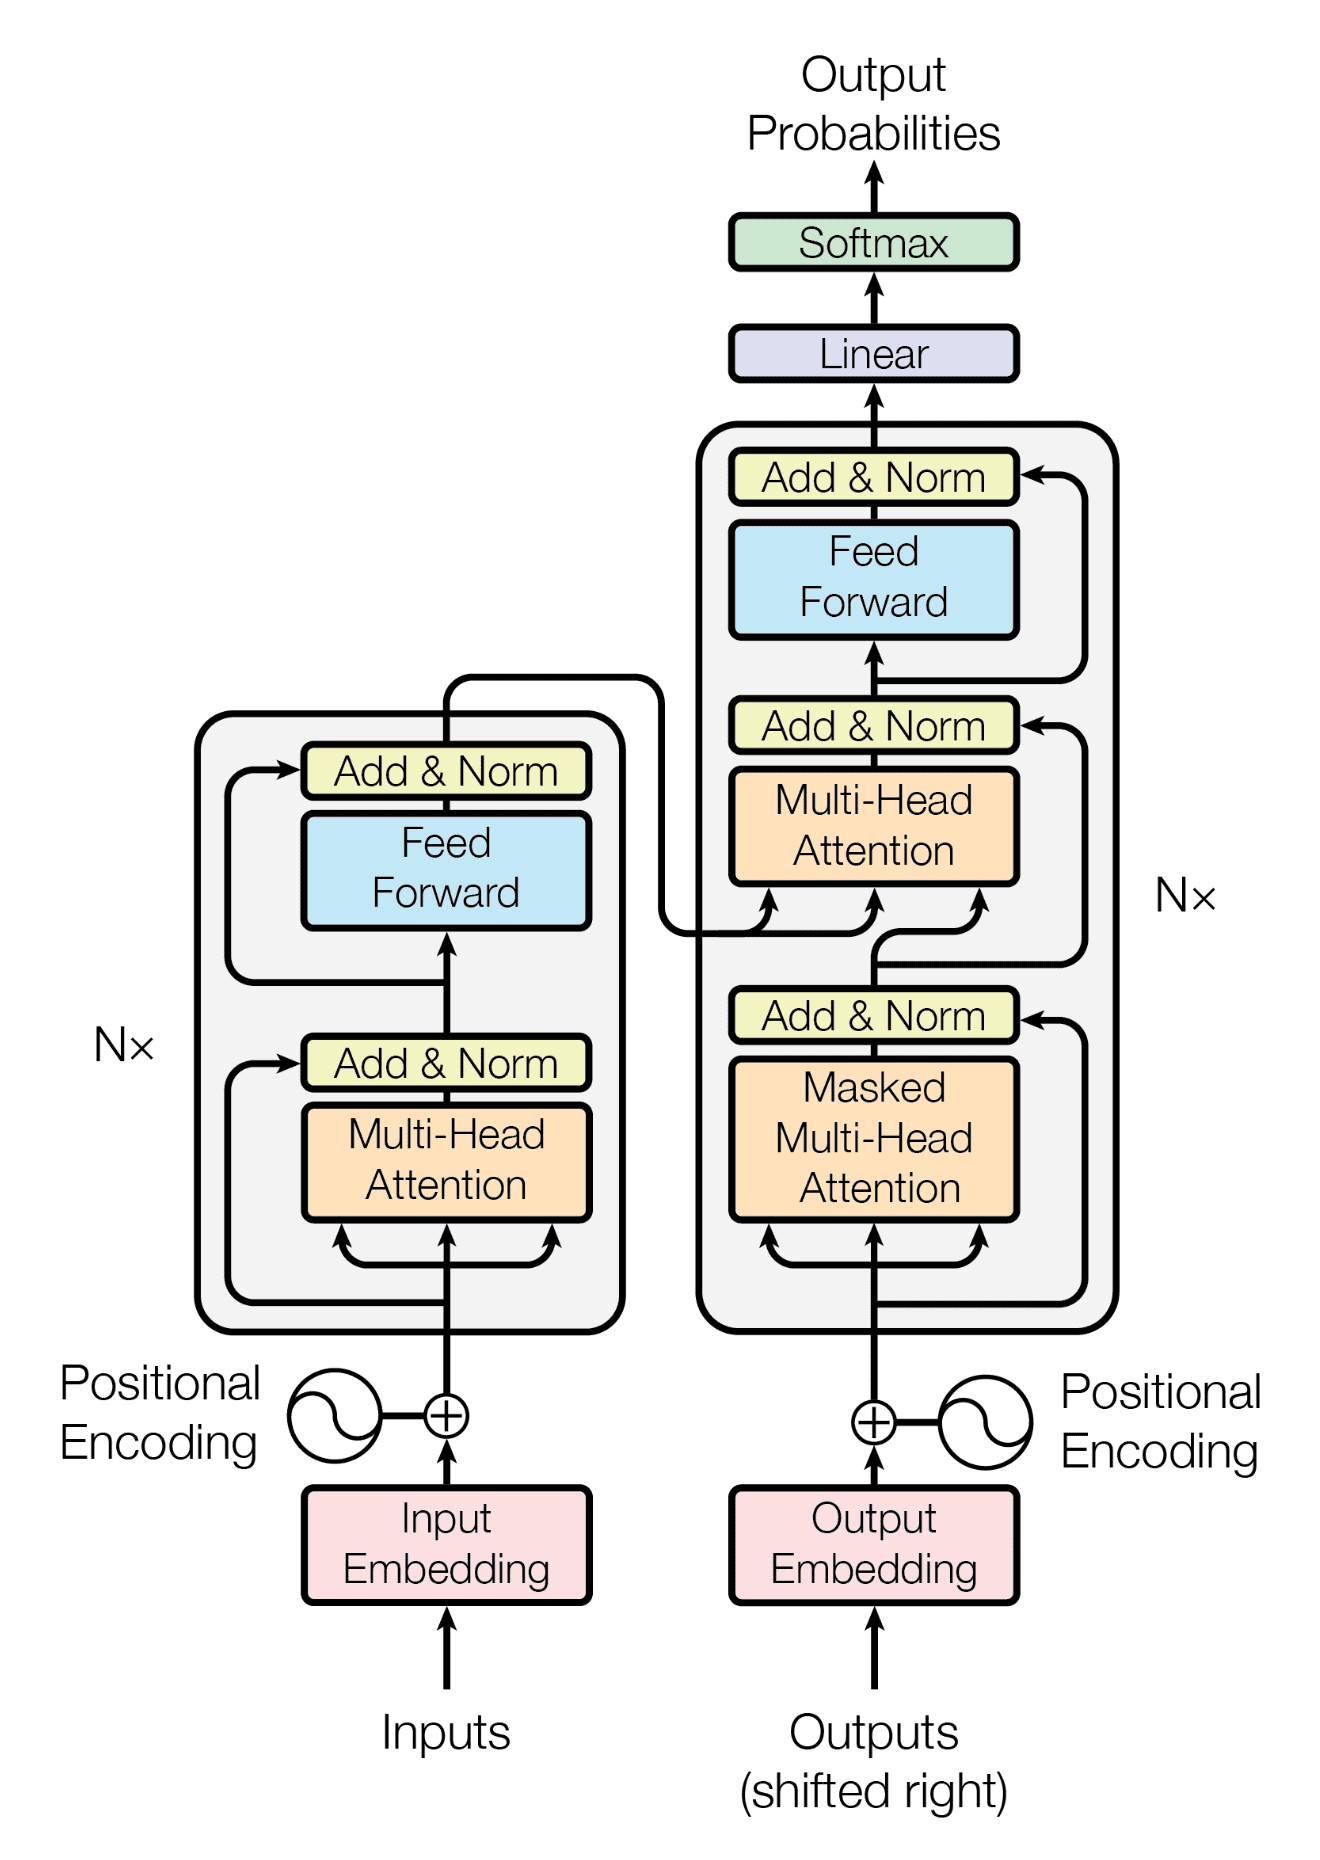
\includegraphics[width=0.5\linewidth]{figures/transformers.png}
    \caption{Transformers architecture.}
    \label{fig:transformer}
\end{figure}

In practice, several attention heads run in parallel and their outputs 
are concatenated, allowing the model to attend to different aspects of 
the input at the same time. This multi-head attention sits alongside 
feed-forward layers and residual connections inside each transformer 
block. BERT \cite{devlin2019bert} stacked 12 such blocks in an 
encoder-only configuration, pre-training on masked language modeling 
to produce contextual representations that became the starting point 
for most subsequent NLP work. Encoder-only models excel at 
classification and retrieval but cannot generate text. Generative 
systems require decoder-based models, described in the next section.

\section{Large Language Models}

\subsection{Decoder-Only Generation}

Decoder-only transformers are trained autoregressively: the model 
predicts the next token given all previous tokens, then appends that 
prediction and repeats until the output is complete. A causal attention 
mask enforces this by preventing any position from attending to tokens 
that come after it in the sequence.

Training these models at scale — billions of parameters on trillions 
of tokens — produces systems that can follow instructions and answer 
questions without task-specific fine-tuning. Instruction-tuned variants 
go a step further: after pre-training, the model is refined using 
reinforcement learning from human feedback (RLHF), which adjusts its 
outputs toward responses that human raters judge as correct and helpful.

\subsection{Llama 3.1}

Meta's Llama family is one of the most widely used open-weight 
generative model series. Llama~2 \cite{touvron2023llama2} released 
7B, 13B, and 70B parameter models alongside instruction-tuned variants 
trained via RLHF. Llama~3.1 \cite{meta2024llama3} extended the series 
with a context window of 128,000 tokens, compared to the 4,096-token 
limit of Llama~2. For legal contracts, which routinely span tens of 
thousands of words, this matters: a clause near the end of a document 
remains accessible to the model during generation rather than being 
truncated out of the input. The 8B parameter variant is used throughout 
this thesis.

\subsection{Mistral 7B}

Jiang et al. released Mistral 7B in 2023 \cite{jiang2023mistral}. 
Despite having fewer parameters than Llama~2~13B, it matched or 
exceeded it on most standard benchmarks. Two architectural decisions 
account for this. Grouped query attention shares key and value matrices 
across multiple attention heads instead of computing a separate pair 
for each, which reduces the memory occupied by the key-value cache 
during inference. Sliding window attention limits each token to 
attending within a fixed window of past positions rather than the 
entire sequence, keeping computation cost proportional to the window 
size rather than the full context length. Both choices lower the 
per-token cost of inference without removing the model's ability to 
reason over long passages.

\subsection{4-Bit NF4 Quantization}

A 7B or 8B parameter model stored in 32-bit floating point requires 
roughly 28--32~GB of GPU memory. Quantization reduces this by 
representing weights at lower precision. The NF4 format, introduced 
by Dettmers et al. as part of QLoRA \cite{dettmers2023qlora}, uses 
a 4-bit encoding designed for the weight distributions found in 
transformer models. Rather than dividing the numeric range into 
equally spaced bins as uniform quantization does, NF4 places bins so 
that each one covers an equal fraction of the weight distribution. 
Since transformer weights are approximately normally distributed, this 
reduces the average quantization error.

The practical result is that both Llama~3.1~8B and Mistral~7B fit 
within 6~GB of GPU memory under NF4, making it possible to run either 
model on a single consumer GPU inside a Docker container. Both models 
are loaded in this format throughout the experiments.

\subsection{Limitations of Large Language Models}

Despite their generative capability, large language models have two 
properties that make them unreliable on their own for document-specific 
question answering.

The first is hallucination. When a model does not have enough 
information to answer a question from its training data, it tends to 
generate a plausible-sounding response anyway rather than declining 
to answer. In a legal context this is particularly problematic: a 
confident but fabricated clause interpretation has no value and could 
actively mislead a user.

The second is static knowledge. A model's parameters are fixed at the 
end of training and cannot be updated without retraining. Any document 
the model has not seen during training — such as a specific commercial 
contract — is outside its knowledge entirely. No amount of prompt 
engineering changes this: the model can only reason about content that 
is explicitly present in its input at inference time. Both of these 
properties motivate augmenting the model with a retrieval component 
that supplies the relevant document text directly, which is the 
approach taken in this thesis.

\section{Semantic Embeddings and Vector Retrieval}

\subsection{Sentence Transformers}

BERT produces one embedding per token, but retrieval requires a 
single vector that represents an entire passage. Reimers and Gurevych 
addressed this by fine-tuning BERT with a Siamese network objective 
on sentence pairs annotated for semantic similarity \cite{reimers2019sbert}. 
The resulting model — Sentence-BERT (SBERT) — passes input through 
the transformer and then aggregates the token embeddings into one 
vector via mean pooling. Training with contrastive loss pulls similar 
pairs together in the vector space and pushes dissimilar pairs apart, 
so that nearby vectors correspond to semantically related text 
regardless of exact wording.

The \texttt{all-MiniLM-L6-v2} model used in this thesis belongs to 
this family. It is a 6-layer encoder producing 384-dimensional 
embeddings. Its small size makes offline indexing of a 500+ contract 
corpus fast, and it achieves strong results on semantic similarity 
benchmarks relative to its parameter count.

\subsection{Cosine Similarity}

Similarity between two embedding vectors is measured with cosine 
similarity:

\begin{equation}
    \cos(\theta) = 
    \frac{\mathbf{u} \cdot \mathbf{v}}{\|\mathbf{u}\|\,\|\mathbf{v}\|}
\end{equation}

A value of 1 means the vectors point in the same direction; a value 
of 0 means they are orthogonal. Because cosine similarity depends 
only on direction and not on vector magnitude, it is not affected by 
differences in text length, which would otherwise make longer passages 
appear more similar to the query simply due to their size.

\subsection{Vector Databases}

After a corpus is embedded, retrieval requires finding the most 
similar vectors to a query without scanning every stored document. 
ChromaDB, the vector database used in this thesis, builds an HNSW 
(Hierarchical Navigable Small World) index over the stored embeddings 
\cite{malkov2018hnsw}. HNSW organizes vectors into a multi-layer 
graph where each node connects to its nearest neighbors at each layer. 
A query starts at the top layer and moves greedily toward the target 
vector, descending to lower layers for progressively finer search. 
This produces sub-linear query time with approximate rather than exact 
results, which is acceptable for RAG: retrieving a near-neighbor 
instead of the absolute nearest has no practical effect on answer 
quality.

\section{Document Chunking}

Full contracts can run to hundreds of pages, but language models 
have fixed context windows. Before indexing, each document is 
divided into smaller passages. Chunk size creates a tradeoff: long 
chunks carry more context but dilute the relevant signal with 
surrounding text, while short chunks are precise but may split a 
clause across two segments and lose its meaning. Three strategies 
are compared in this thesis.

\subsection{Fixed-Size Chunking}

Fixed-size chunking splits text into segments of a predetermined 
character or token count. An overlap is added between consecutive 
chunks so that text near a boundary appears in both adjacent 
segments, reducing the chance that a relevant clause is cut in half. 
The method makes no assumptions about document structure and is 
fast to compute, but it splits at arbitrary positions that may fall 
mid-sentence or mid-clause.

\subsection{Recursive Character Splitting}

Recursive splitting tries to cut at natural document boundaries 
before falling back to arbitrary splits. It first attempts to divide 
at paragraph breaks (double newlines), then at single newlines, then 
at sentence boundaries, and only at the character level if the 
resulting segment still exceeds the target size. This produces more 
coherent chunks than fixed splitting by avoiding mid-sentence cuts 
wherever the document structure allows.

\subsection{Semantic Chunking}

Semantic chunking embeds each sentence individually and computes the 
cosine similarity between consecutive sentence embeddings. A boundary 
is inserted wherever the similarity drops below a threshold, 
indicating a shift in topic. The resulting chunks group sentences 
that discuss the same subject, regardless of where paragraph breaks 
happen to fall in the source document. This approach requires running 
the embedding model on every sentence before indexing, making it 
slower than the other two methods, but it can produce cleaner 
boundaries in legal text where topically related clauses are often 
separated by formulaic boilerplate.

\section{Conversational Memory}

Standard RAG treats each query independently. In a multi-turn 
conversation, follow-up questions frequently refer to earlier turns 
— for example, asking ``what does that clause say about liability?'' 
requires knowing what clause was discussed before. Without memory, 
the system cannot resolve such references. Two approaches are 
compared in this thesis.

\subsection{Windowed Memory}

Windowed memory retains the last $k$ question-answer pairs verbatim 
and prepends them to the current query before retrieval. Nothing from 
the retained window is summarized or reinterpreted, so the context 
passed to the model is exact. The cost is that the prompt grows with 
each turn: for a window of $k$ pairs, roughly $k$ times the average 
exchange length is added to every request. In short conversations 
this is not a problem, but in longer sessions the history eventually 
competes with retrieved passages for the model's context window.

\subsection{Summary Memory}

Summary memory replaces the full conversation history with a 
compressed version generated by the language model. After each 
exchange, the model updates a running summary of the conversation. 
Only this summary, rather than the raw history, is included in 
subsequent prompts. This scales to longer conversations without 
growing the prompt unboundedly, but the compression is lossy: details 
that seem unimportant at the time of summarization may become relevant 
in a later turn, and the summary quality depends on the generator 
being used.

\section{Evaluation Metrics}

\subsection{RAGAS}

RAGAS \cite{es2024ragas} provides four metrics for evaluating RAG 
systems automatically, without requiring human annotation. A language 
model makes the internal judgements for each metric.

\textbf{Faithfulness} checks whether each claim in the generated 
answer is supported by the retrieved context. The answer is split 
into individual statements, and each is verified against the context. 
The score is the fraction of statements that are grounded:

\begin{equation}
    \text{Faithfulness} = 
    \frac{|\text{statements supported by context}|}
         {|\text{total statements in answer}|}
\end{equation}

A low faithfulness score indicates that the model is generating 
content not present in the retrieved passages — the characteristic 
failure mode of hallucination.

\textbf{Answer Relevancy} measures how directly the answer addresses 
the question. A set of synthetic questions is generated from the 
answer and compared to the original question using cosine similarity:

\begin{equation}
    \text{Answer Relevancy} = 
    \frac{1}{N}\sum_{i=1}^{N} 
    \cos\!\left(\mathbf{q}_{\text{original}},\, \mathbf{q}_{i}\right)
\end{equation}

where $N$ is the number of generated questions and $\mathbf{q}_i$ 
is the embedding of the $i$-th synthetic question. An answer that 
directly addresses the question will produce synthetic questions 
close in embedding space to the original.

\textbf{Context Precision} measures whether the relevant retrieved 
passages are ranked above the irrelevant ones. It is computed as 
the mean precision at each rank position where a relevant chunk 
appears:

\begin{equation}
    \text{Context Precision@K} = 
    \frac{1}{|R_K|}\sum_{k=1}^{K} 
    \frac{|R_k|}{k} \cdot \mathbb{1}[c_k \in R]
\end{equation}

where $K$ is the number of retrieved chunks, $R$ is the set of 
relevant chunks, $|R_k|$ is the count of relevant chunks in the 
top $k$ results, $|R_K|$ is the total count of relevant chunks 
among all $K$ retrieved results, and $\mathbb{1}[c_k \in R]$ 
is 1 if the chunk at rank $k$ is relevant.

\textbf{Context Recall} measures whether the retrieved passages 
contain all the information needed to produce the reference answer. 
The ground-truth answer is decomposed into statements, and each 
statement is checked against the retrieved context:

\begin{equation}
    \text{Context Recall} = 
    \frac{|\text{ground-truth statements found in context}|}
         {|\text{total ground-truth statements}|}
\end{equation}

\subsection{LLM-as-a-Judge}

RAGAS measures retrieval quality and grounding, but does not assess 
whether the answer is factually correct relative to the ground truth 
or whether it is appropriately concise. For these two dimensions, a 
capable language model scores each answer on a 1--5 scale using a 
structured prompt that includes the question, the reference answer, 
and the system's response. The raw score is normalized to the 
$[0, 1]$ interval:

\begin{equation}
    s_{\text{normalized}} = \frac{s_{\text{raw}} - 1}{4}
\end{equation}

Correctness and conciseness are scored separately. The correctness 
prompt asks whether the answer contains the information in the 
reference without contradiction. The conciseness prompt asks whether 
the answer is appropriately brief without dropping necessary detail.

Zheng et al. \cite{zheng2023judging} validated single-answer LLM 
scoring against human judgements on MT-Bench and reported agreement 
above 80\%, establishing it as a practical substitute for human 
evaluation at the scale of a systematic experiment.


    \chapter{Dataset and Tools}
\label{chap4}

This chapter describes the data and the software used to build the system. It first presents the CUAD contract dataset that the system retrieves over and from which the evaluation questions are drawn, including its format and the properties that affect how the results should be interpreted. It then introduces the main libraries and frameworks used in the implementation, from the retrieval and generation stack through to the observability and evaluation tools.

\section{The CUAD Dataset}

CUAD (Contract Understanding Atticus Dataset) was introduced by Hendrycks et al.\ \cite{hendrycks2021cuad} as a large-scale benchmark for machine learning on legal contracts. It contains 510 commercial contracts collected from SEC-EDGAR, the public filings database of the U.S.\ Securities and Exchange Commission. Expert lawyers labelled each contract against 41 clause categories that practitioners commonly flag during contract review, including Governing Law, Non-Compete, IP Ownership Assignment, Expiration Date, and Termination for Convenience, among others. The dataset contains more than 13{,}000 manually created annotations in total. Of the 41 categories, 33 require a yes/no answer indicating whether a given clause exists in the contract, while the remaining 8 require an extractive answer such as a state name, a date, or an entity name. This distinction matters for evaluation: the system must handle both the detection of a clause and the extraction of its exact wording.
\subsection{Data Format}

CUAD follows the SQuAD extractive reading comprehension format \cite{rajpurkar2016squad}. Each record pairs a question with a passage from one contract, and the expected answer is a verbatim span extracted from that passage. A boolean field \texttt{is\_impossible} marks whether the queried clause is absent from the contract, enabling evaluation of the system's ability to recognise unanswerable questions. Alongside the annotated JSON file, the dataset distributes all 510 contract texts as plain text files.

\subsection{Usage in This Thesis}
\label{sec:question-sampling}
The 510 contract texts were loaded, split into chunks, and stored in three separate ChromaDB vector databases, one per chunking strategy. The chunking strategies themselves are described in
Chapter~\ref{chap5}.

For evaluation, a stratified random sample of questions was drawn from the dataset
annotations. The sample consisted of 20 questions with a fixed random seed to ensure
reproducibility: 70\,\% were answerable questions (\texttt{is\_impossible=False}) and the remaining
30\,\% were unanswerable (\texttt{is\_impossible=True}). This split ensures that the
evaluation covers both the system's ability to extract the relevant clause text and its
ability to correctly decline when no matching clause exists.

Before each question is submitted to the pipeline, the title of the corresponding
contract is prepended. This allows the retrieval step to focus on the correct
document rather than searching across all 510 contracts simultaneously.

\subsection{Dataset Limitations and Evaluation Considerations}

Working with CUAD in an automated evaluation context revealed several properties of
the dataset that affect how results should be interpreted.

\textbf{Non-conversational question format.}
Every question in CUAD follows a fixed boilerplate template: ``Highlight the
parts (if any) of this contract related to `[Category]' that should be reviewed by a
lawyer. Details: [description].'' This is a legal review instruction, not a natural
question. When RAGAS computes Answer Relevancy, it generates reverse questions from
the system's answer and compares them to the original question using embeddings.
Because the language model answers as if the question were a factual query, the
reverse questions end up semantically distant from the CUAD boilerplate, and the
metric penalises the answer even when it is factually correct. This reflects a
structural mismatch between the CUAD format and the RAGAS evaluation methodology,
not a failure of the system, and it should be kept in mind when interpreting Answer
Relevancy scores.

\textbf{Semantic gap between category names and clause text.}
CUAD category names are short, standardised labels (\textit{Expiration Date},
\textit{Minimum Commitment}, \textit{Governing Law}), whereas the corresponding text
in contracts uses varied legal phrasing: a contract may express expiration as
\textit{``shall terminate upon 90 days written notice''}, or state the governing law
as \textit{``construed in accordance with the laws of the State of Delaware''}. These
pairs are legally equivalent but semantically distant in embedding space, so a
semantic-only retriever can miss the relevant clause even when it is present.This motivated the addition of hybrid retrieval, in which a BM25 keyword index runs alongside the dense retriever and its queries are expanded with legal synonyms for each clause category. Both are described in detail in Chapter~\ref{chap5}.


\textbf{Structured data and annotation quirks.}
Some ground truth answers in CUAD are formatted as tables containing payment
schedules with redacted amounts. Tabular content with few meaningful tokens embeds
poorly and is difficult for any semantic retriever to rank highly. Additionally,
CUAD annotators occasionally marked a termination clause as the ground truth for an
\textit{Expiration Date} question in contracts that carry no fixed expiration date.
In such cases the question and its own ground truth are semantically misaligned,
which can produce misleading Context Recall scores. Both issues are properties of
the dataset rather than the retrieval system.


\section{Implementation Tools}

This section introduces the main libraries and frameworks used to implement the system, grouped by their role in the pipeline: orchestration, storage and retrieval, generation, the user interface, observability, and evaluation.

\subsection{LangChain}

LangChain \cite{chase2022langchain} is a Python framework for building applications
around language models. It provides abstractions for document loading, text
splitting, vector stores, prompt templates, and retrieval chains. In this project,
LangChain handles the entire pipeline: loading the contract files, splitting them
using three different strategies, interfacing with the ChromaDB vector stores,
constructing the prompt templates for question answering and conversation
condensation, and connecting all components through its expression language.

\subsection{ChromaDB}

ChromaDB \cite{chroma2023} is an open-source vector database designed for local
deployment. It stores document embeddings in an HNSW index \cite{malkov2018hnsw},
which supports approximate nearest-neighbour search in sub-linear time. Embeddings
and metadata are persisted to disk between runs. Three separate databases were
created for this project, one for each chunking strategy, so that each experimental
configuration queries its own index and results across configurations remain
directly comparable.

\subsection{Hugging Face Transformers and bitsandbytes}

The Hugging Face Transformers library \cite{wolf2020transformers} was used to load
Llama~3.1~8B Instruct and Mistral~7B Instruct locally from the Hugging Face Hub.
Both models were loaded with 4-bit NF4 quantization via bitsandbytes
\cite{dettmers2022qlora}, reducing memory consumption from approximately 16\,GB in half precision
to roughly 5\,GB per model with minimal quality loss on extractive tasks. Model
weights are distributed across the available GPU automatically. Each model is
subsequently wrapped so that the tokenizer's native chat template is applied
correctly, ensuring the instruction-tuned model receives the expected input format
without echoing the prompt back into its output.


\subsection{Sentence Transformers}

All document chunks and queries were embedded using the all-MiniLM-L6-v2 model from
the Sentence Transformers library \cite{reimers2019sbert}. The model produces
384-dimensional vectors optimised for semantic similarity tasks including passage
retrieval. It was selected for its low computational cost relative to larger
alternatives while still providing reliable retrieval quality for English legal text.

\subsection{BM25 Keyword Retrieval}

In addition to semantic search, the system uses BM25 \cite{robertson2009bm25} for keyword-based retrieval. As noted earlier in this chapter, semantic search can fail when the query and the contract text use different but legally equivalent phrasing. BM25 bridges this gap by matching exact and near-exact terms regardless of semantic distance. The BM25 index is built from the documents stored in the active vector database, and its results are merged with the semantic search hits before being passed to the LLM.

\subsection{Langfuse}

Langfuse \cite{langfuse2023} is an observability platform for LLM applications.
Each call to the RAG pipeline creates a trace that records the user's question, the
reformulated retrieval query, the retrieved chunks, the generated answer, and the
latency of each processing step. In this thesis, Langfuse Cloud is used during the
experimental evaluation to collect per-configuration metrics such as generation
latency and token consumption across all six pipeline configurations, enabling a
direct comparison between the two language models and the three chunking strategies.


\subsection{Streamlit}

Streamlit \cite{streamlit2019} is a Python library for building interactive web
applications. It was used to develop the main user-facing interface of the system:
a browser-based chat application where a user can select a chunking strategy, a
language model, and a memory type, and then hold a natural-language conversation
with the RAG pipeline about the loaded contracts. This interface is the primary
deliverable of the thesis, providing direct access to the system without requiring
any programming knowledge. Language models and vector stores are cached so that
switching one configuration option does not trigger a full reload of the pipeline.


\subsection{Docker}

The full application is containerised with Docker. A dedicated configuration file
installs PyTorch with CUDA support first, then all remaining dependencies. The web
interface is exposed on a fixed port. Langfuse Cloud is accessed through API keys
supplied as environment variables, so no local observability service runs alongside
the container. Containerisation ensures the environment is fully reproducible across different
machines.

\subsection{RAGAS}

RAGAS \cite{es2024ragas} is an evaluation library built specifically for RAG
systems. It computes Faithfulness, Answer Relevancy, Context Precision, and
Context Recall automatically using a judge language model, without requiring manual
annotation of each response. The evaluation pipeline collects the system's answers
and the retrieved context, passes them to the RAGAS evaluator, and writes the
per-question scores together with their averages to a timestamped CSV file for
further analysis.


    \chapter{System Design and Methodology}
\label{chap5}

This chapter describes how the components introduced in Chapters~\ref{chap3}
and~\ref{chap4} are assembled into a working system and how the experimental
evaluation is structured. The theoretical background for the transformer
architecture, semantic embeddings, vector retrieval, and the evaluation metrics
was established in Chapter~\ref{chap3}, and the tools used to implement them were
described in Chapter~\ref{chap4}. This chapter focuses on the specific design
decisions made when connecting those components: the chunking strategies and their
parameters, the retrieval architecture, the prompt design, and the evaluation
protocol. The interactive application and the conversational memory strategies it
exposes are presented separately in Chapter~\ref{chap_app}.

\section{System Architecture Overview}

The system follows a retrieve-then-generate pipeline with conversational memory. A
user submits a question through the web interface. If the conversation has prior turns,
the question is first reformulated into a standalone query that can be understood
without the history. The reformulated query is sent to the retrieval layer, which
fetches the most relevant contract passages from the vector database using a
combination of dense semantic search and BM25 keyword matching. The retrieved
passages, the conversation history, and the original question are passed as context to
the language model, which generates a grounded answer. The answer is returned to the
user and stored in memory for the next turn.

The pipeline runs entirely locally. Both language models run on the host GPU with
4-bit NF4 quantization. The vector databases, the embedding model, and the BM25
index all operate on the same machine without external API calls. Langfuse Cloud
records per-request retrieval and generation latency and token counts for each query
issued during the evaluation.

\section{Document Indexing Pipeline}

This section describes how the contract corpus is prepared for retrieval: how the raw contract files are loaded, how they are split into passages under each of the three chunking strategies, and how the resulting chunks are embedded and stored in the vector databases.

\subsection{Contract Loading}

The 510 CUAD contracts are stored as plain text files. They are loaded using
LangChain's directory loader, which reads all text files from the data directory into
document objects that carry the source file path as metadata. This path is used later
by the retrieval layer to filter results to a specific contract when the user names one.

\subsection{Chunking Strategies}

Full contracts can run to hundreds of pages, but language models have fixed context windows, so each document is divided into smaller passages before indexing. Chunk size is a tradeoff: long chunks carry more context but dilute the relevant signal with surrounding text, while short chunks are precise but may split a clause across two segments and lose its meaning. Three strategies were implemented and compared, each applied to the full contract corpus.

\textbf{Fixed-size chunking} first splits the text at paragraph boundaries (double-newline separators), then groups adjacent paragraphs into chunks of up to 1,000 characters with a 200-character overlap between consecutive chunks. The overlap ensures that text near a boundary appears in both adjacent segments, reducing the chance that a relevant clause is cut in half. Because every split point is a paragraph break, a chunk edge does not fall in the middle of a sentence, so the limitation of the method is size control rather than boundary quality. It is fast to compute, but since it uses only this single separator, a paragraph that already exceeds 1,000 characters is kept whole rather than divided further. About a fifth of the chunks in the fixed collection are therefore larger than the target, the largest reaching nearly ten thousand characters, and these oversized chunks combine several clauses, which dilutes the relevant text when they are retrieved.


\textbf{Recursive character chunking} uses the same 1{,}000-character target and 200-character overlap, but tries to cut at natural boundaries before resorting to arbitrary splits: it attempts paragraph breaks first, then single newlines, then spaces, and only splits mid-text when a segment still exceeds the target size. Because a long paragraph is divided at the finest available boundary rather than kept whole, recursive chunking keeps every chunk close to the target size, whereas fixed-size splitting leaves long paragraphs as single oversized chunks.

\textbf{Semantic chunking} does not use a fixed size target. The embedding model computes the similarity between each pair of adjacent sentences, and a chunk boundary is placed wherever this similarity drops sharply, indicating a topic shift. The resulting chunks group sentences that discuss the same subject, so chunk sizes vary with the content of each contract section. This requires embedding every sentence before indexing, which makes it slower than the other two methods, but it can produce cleaner boundaries in legal text where topically related clauses are separated by formulaic boilerplate. The implementation uses LangChain's \texttt{SemanticChunker} with the default percentile breakpoint method: a boundary is placed wherever the cosine distance between two adjacent sentence embeddings exceeds the 95th percentile of all such distances measured within the document.


\subsection{Vector Database Construction}

After chunking, each collection is embedded with the all-MiniLM-L6-v2 model and
stored in a separate ChromaDB database. The three databases are built once and
persisted to disk. During all subsequent retrieval, they are loaded directly without
re-embedding. Each database functions as an independent index, so switching the
chunking strategy changes only which database is queried, with no other modification
to the pipeline.

\section{Retrieval Architecture}

This section describes how the system selects the passages passed to the language model. Retrieval combines dense semantic search with BM25 keyword matching, adds contract-specific routing so that each query is scoped to the named contract, and reformulates follow-up questions before searching.

\subsection{Dense Semantic Search}
The dense side of retrieval queries the ChromaDB index built for the active chunking strategy. The retrieval query, stripped of the CUAD boilerplate, is embedded with the same all-MiniLM-L6-v2 model used at indexing time, and the index returns the chunks whose embeddings are closest to the query in cosine similarity.

Because every question is scoped to a single named contract, the search is run over a large candidate pool and then filtered to that contract. For each query the index returns a pool of $k \times 10$ chunks, which are filtered to the chunks whose source path matches the named contract. The pool has to be large because the filter discards everything belonging to the other 509 contracts, and a smaller pool would frequently leave too few chunks from the target contract to fill the retrieval budget. With $k = 10$, 100 candidates are scored before filtering. The number of retrieved chunks $k$ is configurable from the Streamlit interface, and $k = 10$ was used for all six configurations in the automated evaluation. The value was chosen to balance retrieval recall against generation cost. A smaller $k$ risks excluding the relevant clause, especially given the vocabulary gap between the standardised CUAD category names and the wording used in the contracts, whereas a larger $k$ lengthens the input, raising generation latency and exposing the model to long-context degradation.

Scoping the search to one contract also removes the main reason a diversity-aware reranker would otherwise be needed. A single contract repeats boilerplate definitions and recurring cross-references, so a plain similarity search can return several near-duplicate passages. The contract-scoped pool combined with the keyword retriever described next, and the deduplication applied when the two result lists are merged, spread the final selection across different parts of the contract rather than returning repeated copies of the single strongest match.


\subsection{BM25 Keyword Retrieval and Hybrid Merging}

As discussed in Chapter~\ref{chap4}, semantic search alone fails when the query and the contract text use legally equivalent but semantically distant phrasing. A BM25 keyword index is built from the same document collection as the vector database and runs alongside the semantic retriever on every query. Running it unconditionally ensures the keyword bridge fires even when semantic search already returned enough passages, since the relevant clause may be worded too differently from the category name for the embedding model to rank it highly. To extend BM25 further, each CUAD category name is paired with a set of legal synonyms. When the query contains a recognised category, the BM25 query is expanded with the corresponding terms before retrieval. For example, a query for \textit{Expiration Date} is expanded with terms such as \textit{terminate}, \textit{termination}, \textit{expire}, \textit{notice period}, and \textit{duration}. This bridges the vocabulary gap between the standardised CUAD label and how the corresponding clause is actually written in practice. The semantic retriever keeps the clean category-and-details query so that embeddings are not diluted by the extra terms.

Results from both retrievers are merged into a single list by interleaving, with
duplicates removed, and trimmed to the target of 10 passages.

\subsection{Contract-Specific Retrieval}

CUAD evaluation questions always refer to a specific named contract. The system detects the contract name from the question, either from a quoted filename or from a human-readable title enclosed in quotes, and filters the semantic search results to passages whose source path matches that contract. A BM25 index is then built over that contract's passages alone and queried with the synonym-expanded query, so both retrievers contribute on every contract-scoped question rather than BM25 acting only as a fallback.


For clause categories that always appear near the top of a contract, such as the document title, the names of the parties, and the agreement date, vector search is bypassed entirely. The first few passages of the matching file are read directly from disk. Vector search is unreliable for these categories because the relevant text typically consists of proper nouns and formatting rather than semantically meaningful prose.

\subsection{Query Reformulation}

Before retrieval, CUAD's fixed boilerplate, \textit{``Highlight the parts (if any)
of this contract related to `[Category]' that should be reviewed by a lawyer. Details:
[description]''}, is stripped from the question. The retrieval query is reduced to
the clause category name and the details description only, giving the vector store a
cleaner signal. The stripped query is used for semantic search; for BM25, the same
query is additionally expanded with the category synonyms.

\section{Conversational RAG Chain}

This section describes the chain that ties retrieval and generation together for multi-turn use: how a follow-up question is condensed into a standalone query before retrieval, and the prompt that instructs the model to answer extractively from the retrieved excerpts.

\subsection{Question Condensation}

Follow-up questions in a conversation often contain unresolved references to earlier
turns, for example \textit{``What about the termination conditions?''} asked after a
question about a different clause. The retriever has no memory, so such references
must be resolved before retrieval. At the start of each turn where prior history
exists, the language model is prompted to rewrite the current question as a
self-contained query using the conversation history. The condensation prompt is shown
in Figure~\ref{fig:condense_prompt}.

\begin{figure}[h!]
    \centering
    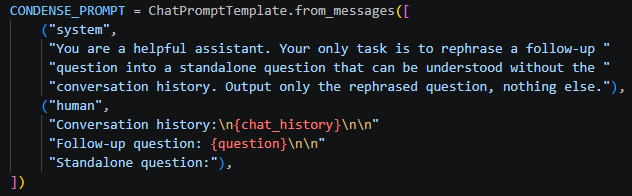
\includegraphics[width=0.84\linewidth]{figures/condense_prompt.png}
    \caption{Question condensation prompt used to resolve follow-up references before retrieval.}
    \label{fig:condense_prompt}
\end{figure}

\subsection{Question Answering Prompt}

The main prompt instructs the model to act as a legal assistant performing extractive question answering. It specifies that each retrieved excerpt is labelled with its source filename, and that if the question names a specific contract, only excerpts from that contract may be used. The prompt defines how to interpret CUAD-style category questions and gives explicit rules for categories such as \textit{Document Name}, \textit{Parties}, and \textit{Governing Law}. It also tells the model when to decline: a fixed not-found phrase must be used when the retrieved excerpts contain no clause related to the requested category, but if a related clause is present without the exact value asked for (a date, an amount, a duration), the clause itself must be quoted rather than refused. Using a fixed phrase rather than free-form refusal makes it straightforward to detect unanswerable responses programmatically during evaluation. Two further rules constrain answer style: the model is told to commit to the single most relevant quote rather than list possibilities with hedging language, and to quote only the minimal span that answers the question rather than reproduce the whole excerpt. The full system message is shown in Figure~\ref{fig:qa_prompt}.

%Both rules target failure modes observed in earlier runs, where correct answers were scored as refusals because of evasive phrasing, or as non-concise because the model included surrounding boilerplate. The full system message is shown in Figure~\ref{fig:qa_prompt}.


\begin{figure}[h!]
    \centering
    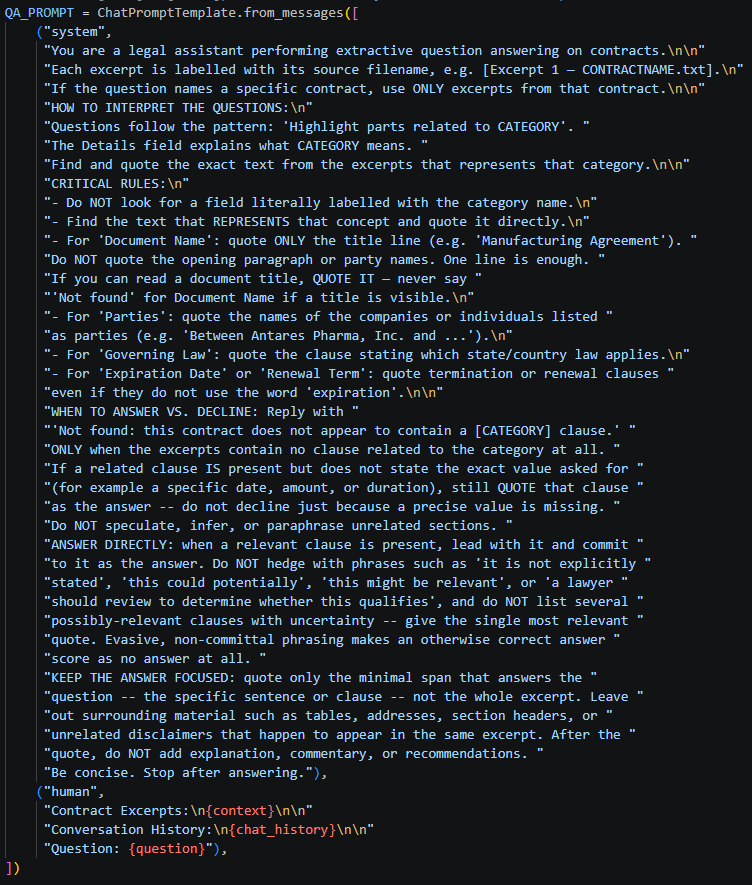
\includegraphics[width=\linewidth]{figures/qa_prompt2.png}
    \caption{Question answering prompt used in all six experimental configurations.}
    \label{fig:qa_prompt}
\end{figure}

\section{Experimental Configurations}

The three chunking strategies and two language models produce six configurations evaluated in the automated experiment. All six are run on the same question set under identical retrieval and prompt conditions. Table~\ref{tab:configs} lists the configurations. Conversation memory is deliberately excluded from this cross: because the automated evaluation resets the conversation history before each question, the windowed and summary strategies produce identical outputs in this
setting and would add no information to the quantitative comparison. They are instead evaluated separately, through a manual multi-turn test in the interactive application, in Chapter~\ref{chap_app}.


\begin{table}[h!]
\centering
\begin{tabular}{cll}
\hline
\textbf{Config} & \textbf{Chunking Strategy} & \textbf{Language Model} \\
\hline
1 & Fixed     & Llama 3.1 8B \\
2 & Fixed     & Mistral 7B   \\
3 & Recursive & Llama 3.1 8B \\
4 & Recursive & Mistral 7B   \\
5 & Semantic  & Llama 3.1 8B \\
6 & Semantic  & Mistral 7B   \\
\hline
\end{tabular}
\caption{The six experimental configurations evaluated in this thesis.}
\label{tab:configs}
\end{table}

\newpage
\section{Evaluation Methodology}

This section describes the protocol used to evaluate the six configurations: how the question sample is drawn, how RAGAS and the LLM-as-a-Judge produce their scores, and how the no-retrieval baseline is run for comparison.

\subsection{Question Sampling}
\label{sec:eval-sampling}

The evaluation uses the 20-question stratified sample described in Section~\ref{sec:question-sampling}. The same set is used for all six configurations and the
no-retrieval baseline, so all comparisons are made on identical inputs.


Before each question is submitted, the title of the corresponding contract is
prepended in the format \textit{``Contract Title'' question text}. This triggers
the contract-specific retrieval and prevents the pipeline from searching across all 510 contracts for each query.

\subsection{RAGAS Evaluation}

For each configuration, the system's answers and retrieved context are passed to the RAGAS evaluator. RAGAS requires an external language model to make the judgements for Faithfulness, Answer Relevancy, Context Precision, and Context Recall. The evaluator used in this thesis is OpenAI's GPT-4o-mini, accessed through the OpenAI API. GPT-4o-mini was chosen because it consistently produces well-formed JSON verdicts for the structured scoring tasks RAGAS requires, at a cost low enough to evaluate the full six-configuration sweep without budget concerns. Any scores returned as null are excluded from the configuration averages.

Unanswerable questions are excluded from RAGAS evaluation. When the ground truth is
empty, Context Recall is zero by definition regardless of what was retrieved, and
Faithfulness becomes ill-defined. Including these questions would suppress the
averages in a way that does not reflect retrieval quality.

\subsection{LLM-as-a-Judge Evaluation}

Correctness and conciseness are scored by the same external model used for RAGAS.
Correctness is evaluated only for answerable questions, comparing the system's answer
against the CUAD ground truth span on a 1--5 scale. Conciseness is evaluated for all
non-error answers regardless of whether the question is answerable. Both scores are
normalised to the $[0, 1]$ interval using the formula defined in
Chapter~\ref{chap3}. The judge receives the question, the ground truth (for
correctness), and the system's answer, and must respond with a JSON object containing
the score and a one-sentence justification. The correctness and conciseness scoring prompts are shown in Figures~\ref{fig:judge_correctness_prompt} and~\ref{fig:judge_conciseness_prompt}.

\begin{figure}[h!]
    \centering
    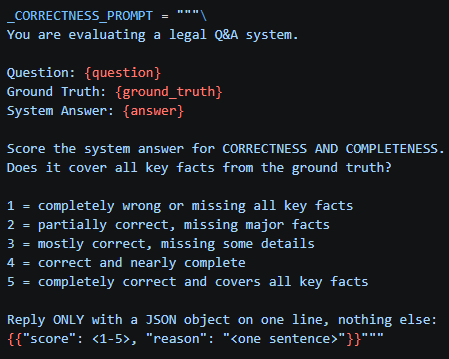
\includegraphics[width=0.6\linewidth]{figures/judge_correctness_prompt.png}
    \caption{LLM-as-a-Judge correctness prompt.}
    \label{fig:judge_correctness_prompt}
\end{figure}

\begin{figure}[h!]
    \centering
    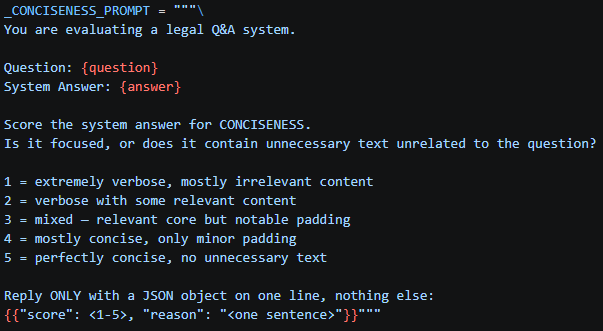
\includegraphics[width=0.8\linewidth]{figures/judge_conciseness_prompt.png}
    \caption{LLM-as-a-Judge conciseness prompt.}
    \label{fig:judge_conciseness_prompt}
\end{figure}

\newpage
\subsection{No-Retrieval Baseline}

To measure the contribution of retrieval, each language model is also run without any retrieved context on the same twenty questions. The model receives only the question and a brief instruction to answer from general legal knowledge or to respond with \textit{``Not found''} if the answer requires reading the specific contract. Since there is no retrieved context, RAGAS metrics are not applicable to the baseline. Correctness and conciseness are scored by LLM-as-a-Judge, allowing a direct comparison of judge correctness between the RAG configurations and the no-retrieval baseline for each language model. This comparison quantifies how much retrieval contributes to answer quality over what the model already knows from training. The baseline prompt is shown in Figure~\ref{fig:baseline_prompt}.

\begin{figure}[h!]
    \centering
    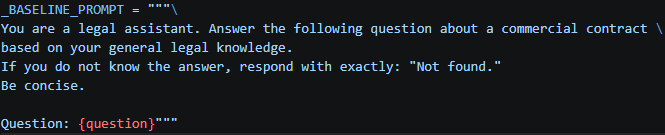
\includegraphics[width=0.88\linewidth]{figures/baseline_prompt.png}
    \caption{No-retrieval baseline prompt.}
    \label{fig:baseline_prompt}
\end{figure}


    \chapter{Experimental Results}


\section{Evaluation Setup}
All six configurations were evaluated using GPT-4o-mini as the external judge for both RAGAS metrics and the LLM-as-a-Judge scores. Each configuration was run on the same stratified 20-question sample described in Section 5.7.1. Fourteen of the twenty questions were answerable (is\_impossible=False) and six were unanswerable. RAGAS metrics were computed only on the answerable subset; Judge Correctness was also restricted to answerable questions; Judge Conciseness was computed for all non-error answers. Results for each question were written to a timestamped CSV file and averaged per configuration. The six unanswerable questions were evaluated manually: for each one, the model's response was inspected to determine whether it correctly acknowledged that the requested information was not present in the contract. A response was counted as correct if it explicitly stated that the answer could not be found, without fabricating a plausible-sounding but unsupported answer. The retriever was configured with $k=10$ chunks per query for all runs. Each configuration was evaluated independently, with no shared conversation history between questions.

\section{Results Overview}


Table~\ref{tab:results} summarizes the mean scores across all six configurations. The highest value in each column is shown in bold.

\begin{table}[ht]
\centering

\label{tab:results}
\resizebox{\textwidth}{!}{%
\begin{tabular}{llccccccc}
\toprule
\textbf{Chunking} & \textbf{LLM} & \textbf{Faithfulness} & \textbf{Ans.\ Rel.} & \textbf{Ctx.\ Prec.} & \textbf{Ctx.\ Rec.} & \textbf{Correctness} & \textbf{Conciseness} & \textbf{Latency (s)} \\
\midrule
Fixed     & Llama 3.1 8B  & 0.69 & 0.55 & \textbf{0.89} & 0.84 & 0.71 & 0.80 & 29.9 \\
Fixed     & Mistral 7B    & 0.51 & 0.24 & 0.87          & 0.86 & 0.46 & \textbf{0.90} & 13.7 \\
Recursive & Llama 3.1 8B  & 0.70 & 0.48 & 0.88          & 0.78 & 0.70 & 0.78 & 19.2 \\
Recursive & Mistral 7B    & 0.58 & 0.43 & 0.88          & 0.81 & 0.45 & \textbf{0.90} & \textbf{13.2} \\
Semantic  & Llama 3.1 8B  & \textbf{0.81} & \textbf{0.71} & 0.85 & \textbf{0.89} & \textbf{0.79} & 0.79 & 148.3 \\
Semantic  & Mistral 7B    & 0.46 & 0.37 & 0.85          & \textbf{0.89} & 0.48 & \textbf{0.90} & 52.5 \\
\bottomrule
\end{tabular}%
}
\caption{Mean evaluation scores for all six configurations. Higher is better for all metrics except latency.}
\label{tab:results}
\end{table}

\section{Retrieval Quality}
Context Precision and Context Recall are stable across all six configurations. Precision ranges from 0.85 to 0.89 and recall from 0.78 to 0.89 — a spread of less than 0.1 in both cases. This reflects the fact that all configurations share the same retrieval mechanism: hybrid MMR and BM25 with legal synonym expansion over the same document corpus. The model choice has no effect on what gets retrieved, since retrieval runs before the language model is invoked. Switching chunking strategy changes chunk boundaries, not the retrieval logic.

The one outlier is Context Recall for Recursive+Llama at 0.78, lower than the 0.84–0.89 range seen elsewhere. This is likely a sampling effect: the 20-question sample included several questions whose ground truth spans sit near the boundaries used by recursive splitting for those specific contracts, causing the relevant text to be split across two chunks rather than appearing in a single retrieved passage.

\section{Generation Quality}
The generation metrics — Faithfulness, Answer Relevancy, and Judge Correctness — show wider variation and divide clearly along model lines.

Semantic+Llama produced the best generation scores of all six configurations: Faithfulness 0.81, Answer Relevancy 0.71, Judge Correctness 0.79. It is the only configuration where all three generation metrics exceeded 0.7. The other two Llama configurations scored 0.69–0.70 on Faithfulness but dropped to 0.48–0.55 on Answer Relevancy, suggesting that fixed and recursive chunks frequently include surrounding content beyond the relevant clause, and Llama quotes it rather than isolating the answer.

Mistral shows a different failure mode. Faithfulness ranges from 0.46 to 0.58 across the three chunking strategies — consistently below all three Llama configurations — while conciseness sits at 0.90 regardless of chunking. Mistral produces shorter answers, but those answers are less grounded in the retrieved context and less factually correct. The gap in Judge Correctness is large: Mistral averages 0.45–0.48 against Llama's 0.70–0.79.

Semantic+Mistral is the worst single configuration on Faithfulness at 0.46. The semantic chunks that raised Llama's faithfulness to its peak instead appear to overwhelm Mistral: the model generates a short answer that does not draw on the full content of the longer, topically coherent passage it was given.

\subsection{Unanswerable Questions}

Six of the twenty questions correspond to clauses that are not present in the queried contracts (\texttt{is\_impossible=True}). Because there is no ground-truth answer text to compare against, these questions were excluded from the automated RAGAS and Judge Correctness calculations. Judge Conciseness was still computed automatically, but conciseness alone does not measure whether the model correctly declined to answer; a short hallucination scores as well as a short correct refusal.

The six unanswerable questions were therefore evaluated manually. A response was counted as correct if it ultimately acknowledged that the requested clause was not present in the contract, even if it first discussed adjacent or topically related sections. This rule reflects how the system would be used in practice: surfacing nearby material for a human reviewer to consider is preferable to silently omitting it, provided the model does not falsely claim that the requested clause is present. A response was counted as incorrect if it treated an adjacent clause as the answer or if it concluded that the requested clause might exist when in fact it does not.

Table~\ref{tab:unanswerable} shows the per-configuration results. Across all six configurations, the models handled 33 of 36 unanswerable questions correctly (average 5.5 of 6).

\begin{table}[ht]
\centering
\caption{Manual evaluation of the six unanswerable (\texttt{is\_impossible=True}) questions per configuration.}
\label{tab:unanswerable}
\begin{tabular}{llc}
\toprule
\textbf{Chunking} & \textbf{LLM} & \textbf{Correct / 6} \\
\midrule
Fixed     & Llama 3.1 8B & 4 \\
Fixed     & Mistral 7B   & 6 \\
Recursive & Llama 3.1 8B & 5 \\
Recursive & Mistral 7B   & 6 \\
Semantic  & Llama 3.1 8B & 6 \\
Semantic  & Mistral 7B   & 6 \\
\bottomrule
\end{tabular}
\end{table}

The three failures came from Llama configurations, two of them on the Third Party Beneficiary question. All three failures share the same pattern: the retrieved excerpts contained legally adjacent material, and the model treated similarity in subject matter as a sufficient basis for a positive answer.

Mistral handled every unanswerable question correctly in all three chunking configurations. Its tendency to produce shorter, more cautious responses worked in its favour here, since a short refusal is harder to dilute with adjacent clauses than a longer extractive answer. Llama's more elaborate response style, which improved its scores on answerable questions, made it more prone to constructing a partially supported argument when the correct answer was that the clause was absent.



\section{Effect of Chunking Strategy}
For Llama, moving from fixed to semantic chunking raises Faithfulness from 0.69 to 0.81 and Judge Correctness from 0.71 to 0.79. The gain in Answer Relevancy is larger, from 0.55 to 0.71. Recursive chunking sits between the two on most metrics. This pattern matches the theoretical expectation: semantic chunks group sentences by topic, so the retrieved passage is more likely to consist entirely of the relevant clause rather than a mix of the clause and surrounding boilerplate. Llama generates more precise answers when the context is cleaner.

For Mistral, the pattern reverses. Semantic chunking produces the lowest Faithfulness score (0.46) of all six configurations. Mistral scores higher on fixed (0.51) and recursive (0.58) chunking — shorter, more constrained passages that leave less room for the model to drift from the retrieved content.

The best chunking strategy is therefore model-dependent. Semantic chunking is clearly preferable when Llama is the generator but harmful when Mistral is used. A deployment decision that fixes the language model should adjust the chunking strategy accordingly.
\section{Effect of Language Model}
Llama 3.1 8B outperforms Mistral 7B on every generation quality metric in every chunking configuration. The average gap in Faithfulness across the three chunking strategies is approximately 0.18 points, in Judge Correctness approximately 0.25 points, and in Answer Relevancy approximately 0.20 points.

Mistral compensates with speed. It generates answers in 13–14 seconds regardless of chunking strategy, compared to Llama's 13–148 seconds. For fixed and recursive chunking the difference is small — Mistral runs in 13 seconds and Llama in 19–30 seconds — but for semantic chunking Llama's 148 seconds is more than 11 times slower than Mistral's 52 seconds.

For a legal application where answer quality is the primary concern, Llama 3.1 8B is the better choice. If response time matters more than accuracy — for example, a high-volume screening tool that flags contracts for human review rather than providing relied-upon answers — Mistral with recursive chunking offers reasonable retrieval quality at roughly a third of the generation cost.

\section{Response Latency}
Semantic chunking carries a significant latency penalty for Llama. Fixed and recursive configurations run in 19–30 seconds per query; semantic+Llama takes 148 seconds, nearly five times longer. Semantic chunks are larger on average than fixed or recursive ones, and generation time scales with context length. The same effect is visible for Mistral — semantic chunking raises its latency from 13 to 52 seconds — but the absolute numbers remain more practical.

Semantic+Llama would be unusable in an interactive setting where users expect a response within a minute. It is viable for batch processing, such as overnight evaluation runs or bulk contract analysis, but it cannot be the default configuration for the real-time chat interface. For that use case, Fixed+Llama or Recursive+Llama offer the best balance of quality and speed.

\section{Qualitative Observations}
A recurring pattern in Llama's outputs is the inclusion of surrounding content from the retrieved chunk beyond what the question asked. When a passage contains a relevant clause alongside an unrelated table, address, or liability disclaimer, the model frequently quotes the entire passage rather than extracting the clause. This behaviour explains the Answer Relevancy gap between Llama's fixed/recursive and semantic configurations: with fixed and recursive chunks the answer is correct but verbose, and the verbosity dilutes the relevancy signal.

Faithfulness and correctness can diverge when retrieval fails. If the retrieved passages do not contain the relevant clause, the model generates an answer that is faithful to what it was given — no fabrication relative to the retrieved context — but factually wrong relative to the ground truth. In one evaluation example involving a liability cap clause in the NETGEAR distributor agreement, the system retrieved an infringement limitations passage instead of the cap clause, and concluded that no cap existed. Faithfulness was high; correctness was not. This illustrates that faithfulness alone is insufficient as a quality measure: a system can be perfectly faithful to the wrong context.

The conciseness metric behaved inconsistently for unanswerable questions. When the system correctly identified that a clause was not present, it typically showed the retrieved excerpts it searched before reaching its conclusion. The judge scored these responses as verbose and penalised conciseness, even when the behaviour was appropriate. This is a known limitation of applying a general-purpose conciseness measure to a system designed to show source evidence alongside its conclusions.

\section{Memory Strategy Comparison}
The automated evaluation runs each question in isolation, resetting conversation history before each turn. Both windowed and summary memory are therefore equivalent in that setting. To compare the two strategies in a realistic multi-turn scenario, a fixed sequence of seven questions was run manually through the Streamlit interface — six questions drawn from the CUAD annotations for a random contract that was chosen of the 510 contracts (Sphere 3D Corp consulting agreement), plus one question that references information from a turn before the memory context window.

\subsection{Question Sequence}

The six content questions covered the following CUAD categories: (1) contracting parties, (2) effective date, (3) expiration date of the initial term, (4) governing law, (5) consequences of failing to notify before the term ends, and (6) non-compete restrictions. The seventh question was a meta-question asking the model to recall the first question of the session and the answer it gave, without referencing the contract by name.

Question 6 has \texttt{is\_impossible=True} in the CUAD annotations: the Sphere 3D Corp consulting agreement does not contain a non-compete clause. This question was included to verify that the model correctly declines to answer rather than fabricating a clause. 

\subsection{Windowed Memory Results}

Questions 1 through 6 were answered correctly under windowed memory ($k=5$). The retrieval query at each turn included the full contract filename, which the condense step reconstructed from conversation history, so retrieval remained contract-specific throughout the session (Figures~\ref{fig:memory1} and~\ref{fig:memory2}).

\begin{figure}[h!]
    \centering
    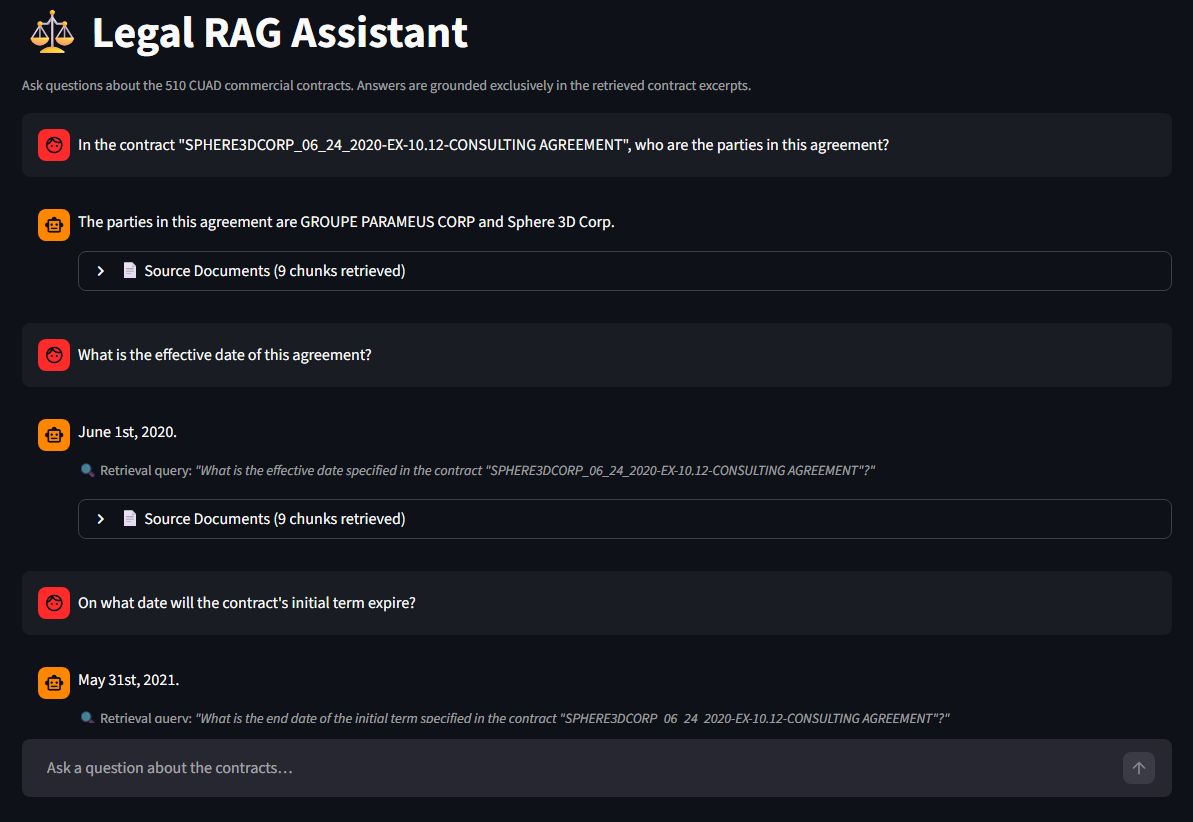
\includegraphics[width=\textwidth]{figures/memory1.png}
    \caption{Windowed memory session — questions 1 to 3.}
    \label{fig:memory1}
\end{figure}

\begin{figure}[h!]
    \centering
    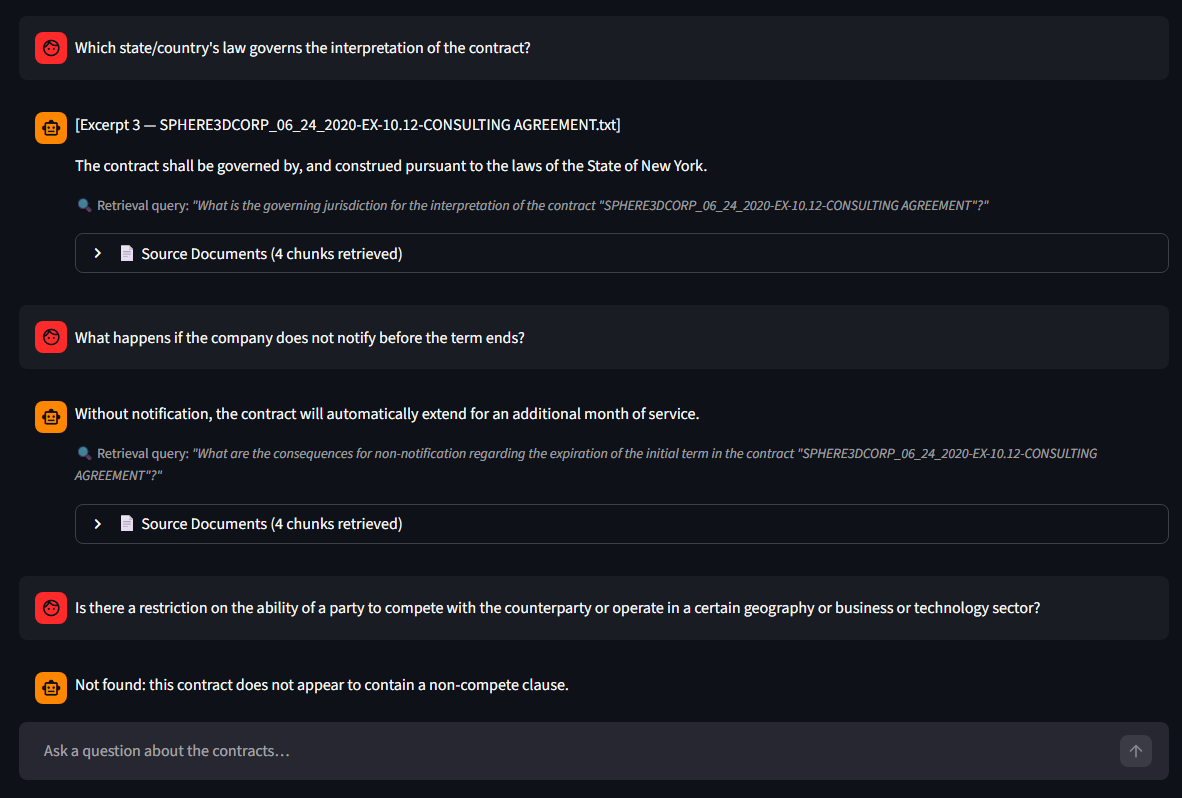
\includegraphics[width=\textwidth]{figures/memory2.png}
    \caption{Windowed memory session — questions 4 to 6.}
    \label{fig:memory2}
\end{figure}

\begin{figure}[h!]
    \centering
    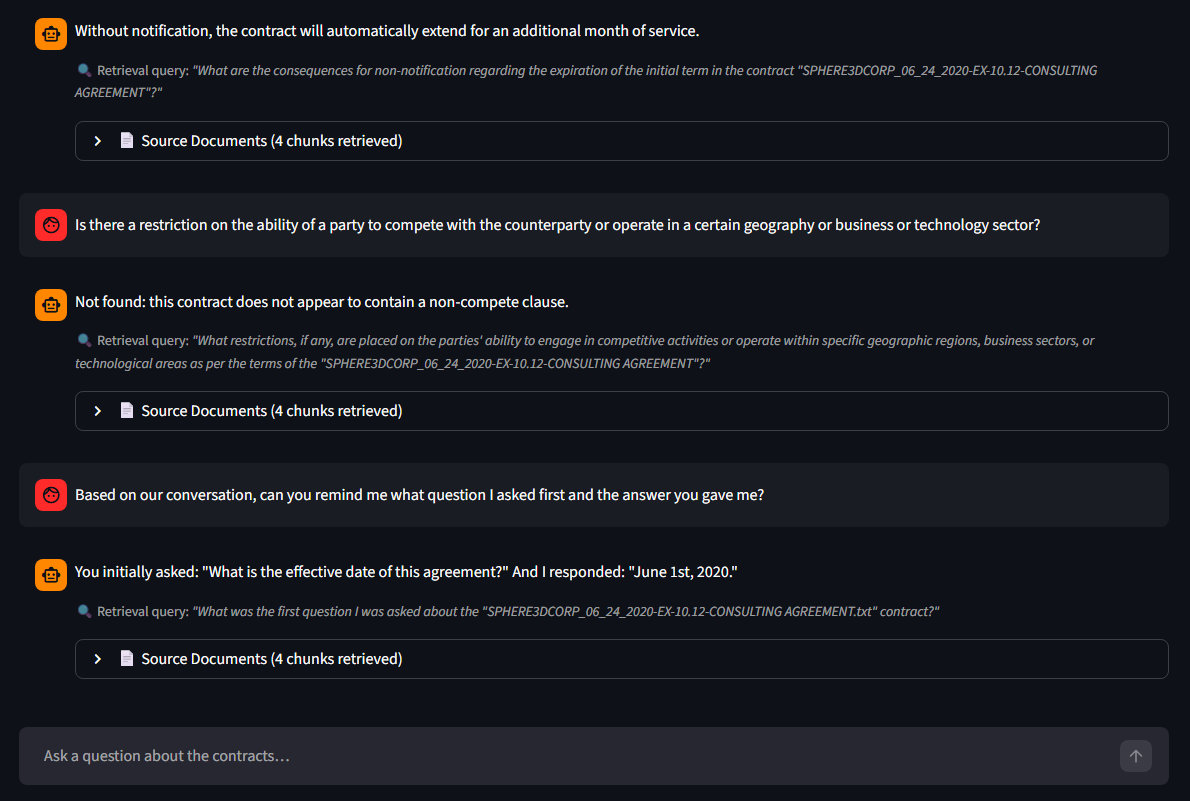
\includegraphics[width=\textwidth]{figures/memory3.png}
    \caption{Windowed memory failure at question 7. The model reports the effective date question as the first question asked, because question 1 (contracting parties) has been evicted from the $k=5$ window.}
    \label{fig:memory3}
\end{figure}

The failure appeared at question 7 (Figure~\ref{fig:memory3}). At that point the conversation history contained six completed turns. The windowed buffer holds only the last five, so question 1 — "In the contract SPHERE3DCORP\_06\_24\_2020-EX-10.12-CONSULTING AGREEMENT, who are the parties in this agreement?" — had been evicted from the context window. When asked to recall the first question of the session, the model identified question 2 ("What is the effective date of this agreement?") as the first, because that was the oldest turn still present in its window. The actual first question and its answer were permanently lost.

\newpage
\subsection{Summary Memory Results}

Under summary memory, the LLM maintains a running compressed summary of the full conversation after each turn. After question 1, the summary includes the fact that the user asked about the contracting parties and that the answer was GROUPE PARAMEUS CORP and Sphere 3D Corp. This summary is never truncated, it is updated incrementally and passed in full on every subsequent turn. When question 7 was asked under summary memory, the model correctly identified question 1 as the parties question and reproduced the correct answer, demonstrating that the information survived across all seven turns.

\begin{figure}[h!]
    \centering
    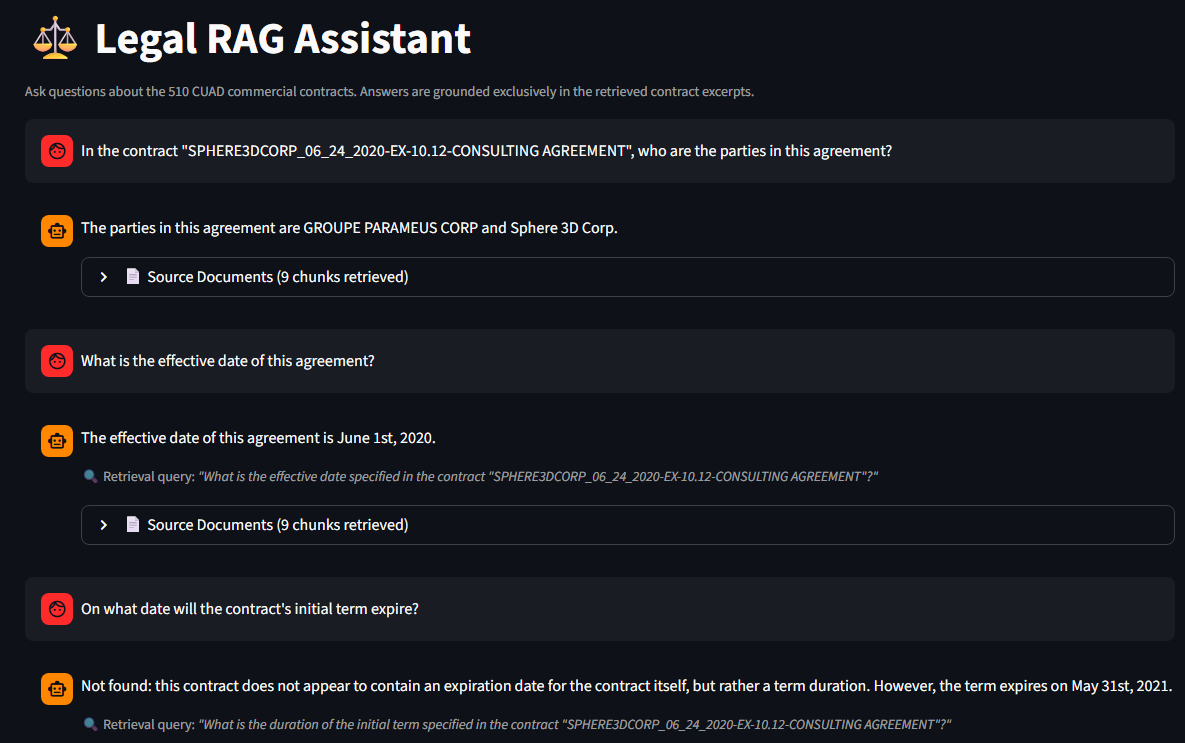
\includegraphics[width=\linewidth]{figures/summary1.png}
    \caption{Summary memory session — questions 1 to 3.}
    \label{fig:placeholder}
\end{figure}

\begin{figure}[h!]
    \centering
    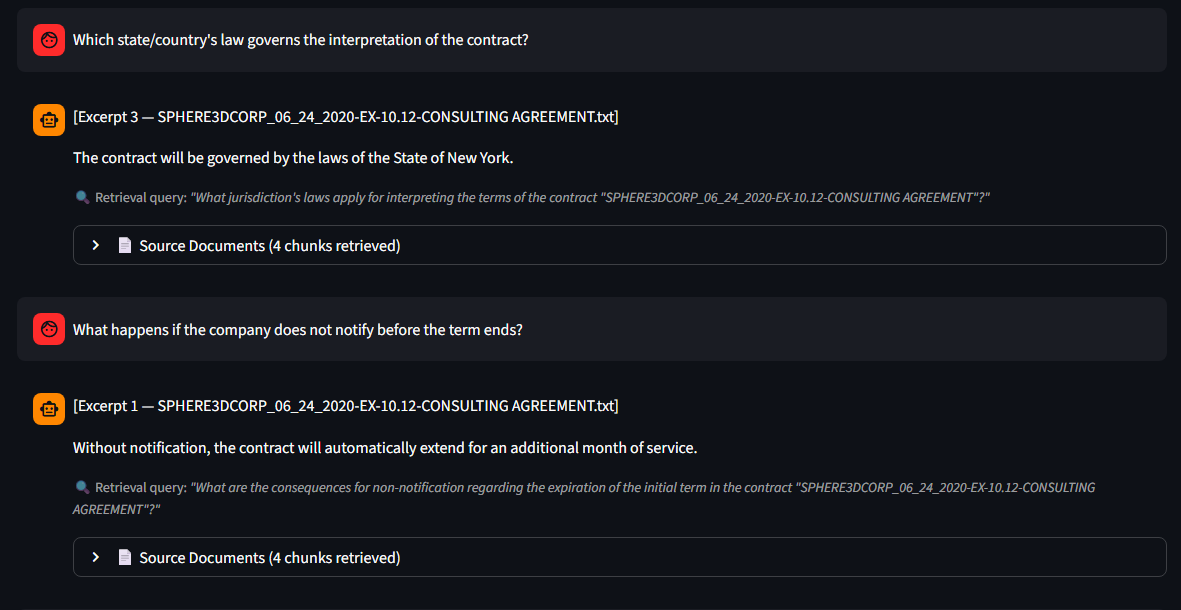
\includegraphics[width=\linewidth]{figures/summary2.png}
    \caption{Summary memory session — questions 4 to 5.}
    \label{fig:placeholder}
\end{figure}


\begin{figure}[h!]
    \centering
    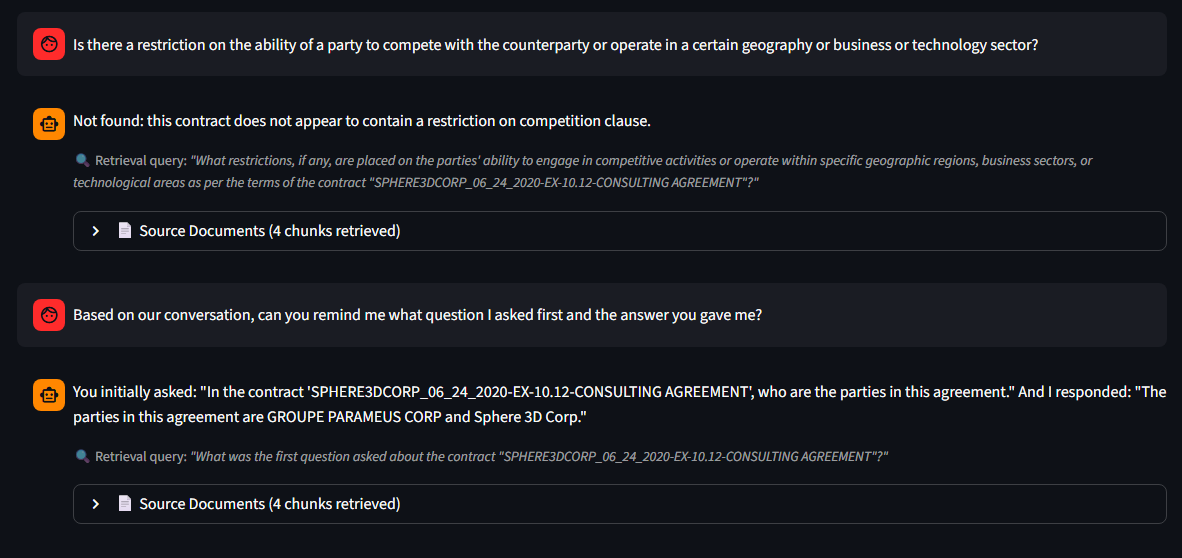
\includegraphics[width=1\linewidth]{figures/summary3.png}
    \caption{Summary memory session — questions 6 to 7.}
    \label{fig:placeholder}
\end{figure}

\newpage

\subsection{Discussion}

In a real case scenario, a user who wants to recall an earlier answer or question can simply scroll through the chat history in the interface. The test was done with this recall question to simply show the difference between the two memory window techniques. A more meaningful test is one where the model must retain context that the user stated about themselves, information that exists only in the conversation and cannot be retrieved from any document. To construct such a test, the first question of the session was modified to include a role declaration: "I am a lawyer representing the Consultant in this matter. In the contract SPHERE3DCORP\_06\_24\_2020-EX-10.12-CONSULTING AGREEMENT, who are the parties?". After five further questions covering the effective date, expiration, governing law, auto-renewal consequences, and non-compete restrictions, the seventh question asked: "Based on our conversation, which party am I representing, and what are their obligations if the company fails to give notice before the term ends?". This question cannot be answered by retrieval alone. The contract does not record who the user represents because that information exists only in Q1, which falls outside the windowed memory buffer at turn seven.

Under windowed memory (Figure ~\ref{fig:windowfinal}), the model answered "you are representing the company" it completely lost the context of the party, it didn't even provide the company name. Q1 had been evicted from the buffer after six turns, and the model had no record of the role declaration. With no grounded context to draw from, it guessed incorrectly. The condense chain also failed to reconstruct the contract filename, producing a vague retrieval query with no contract reference and retrieving ten chunks from multiple contracts.

\begin{figure}[h!]
    \centering
    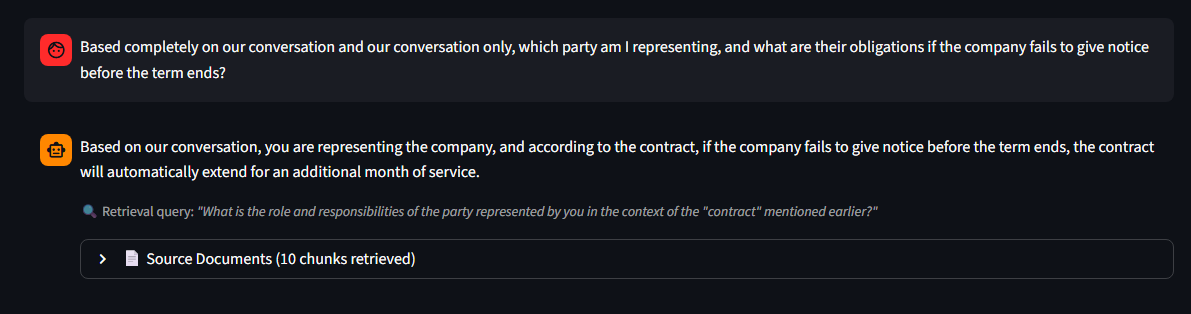
\includegraphics[width=\linewidth]{figures/windowfinal.png}
    \caption{Question 7 under windowed memory ($k=5$) — incorrect identification of the represented party.}
    \label{fig:windowfinal}
\end{figure}

Under summary memory (Figure ~\ref{fig:summaryfinal}), the model identified GROUPE PARAMEUS CORP as the party being represented and described the auto-extension clause as the relevant obligation. The role declaration from Q1 had been captured in the running summary and remained available throughout the session. The condense chain, informed by the richer summary, also generated a precise retrieval query that included the full contract filename, retrieving four targeted chunks rather than ten mixed ones. The phrase "based on our conversation only" was added deliberately to prevent the model from inferring the role from contract content, isolating memory as the only possible source of the answer.

\begin{figure}[h!]
    \centering
    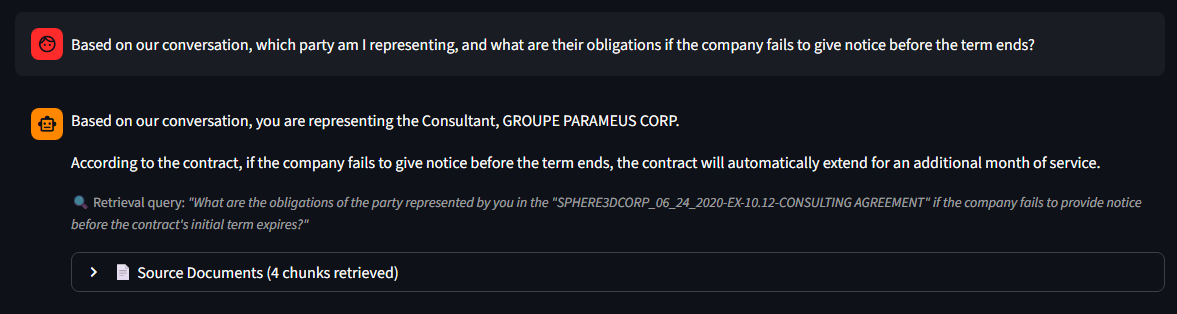
\includegraphics[width=\linewidth]{figures/summaryfinal.png}
    \caption{Question 7 under summary memory — correct identification of the consultant.}
    \label{fig:summaryfinal}
\end{figure}

Windowed memory is simple and guarantees exact verbatim recall of recent turns, but it silently discards older context once the buffer is full. Summary memory avoids this by compressing rather than discarding, at the cost of losing fine-grained verbatim detail in older turns. For long legal sessions that may span many clauses of a single contract, summary memory is the more appropriate choice, since a user may reference a clause discussed several turns earlier without the system having lost all trace of it.



    %\include{chapter...} % προσθέστε όσα χρειάζεται
    \chapter{Conclusion}
\label{chap_last}

This chapter draws together the findings of the thesis. It first summarizes what was built and what the evaluation showed across the six configurations, the no-retrieval baseline, and the memory comparison, and then sets out the main directions for future work that follow from the system's limitations.


\section{Summary and Conclusions}
This thesis built a conversational question answering system for commercial legal contracts and measured how its main design choices affect the quality of the answers. The system retrieves passages from the CUAD corpus with a combination of dense vector search and BM25 keyword matching, routes each query to the named contract, and generates an answer with a locally run language model
under 4-bit quantization. Three chunking strategies and two language models were crossed to give six configurations, each evaluated on the same stratified sample of CUAD questions with four RAGAS metrics and two LLM-as-a-Judge metrics.

The introduction set out two properties that make a language model unreliable on its own for this task: it tends to produce confident but ungrounded answers when it lacks the information, and it cannot access documents it never saw during training. The no-retrieval baseline measured both directly. Without any retrieved context, Llama~3.1~8B reached only 0.36 on Judge Correctness, either declining or describing in general terms where the requested clause usually appears, without recovering the contract-specific facts. Adding retrieval raised its Correctness to 0.77 on average across the three chunking strategies, a gain of roughly 0.41 points. Mistral~7B moved far less, from 0.63 to 0.67, but its higher baseline is misleading: it answers every question with a fluent generic legal template that the judge credits for completeness even though it contains no facts from the specific contract. The retrieval component, not the language model on its own, is what makes the system produce grounded, contract-specific answers.

Retrieval quality was high and stable across all six configurations. Context Precision stayed between 0.91 and 0.95 and Context Recall between 0.87 and 0.96, because every configuration shares the same retrieval mechanism and the choice of language model does not change what is retrieved. The generation metrics varied more and divided along model lines, though by a smaller margin than the model sizes would suggest. Llama~3.1~8B scored higher than Mistral~7B on the generation metrics in every chunking configuration, with an average gap of about 0.16 on Faithfulness and 0.10 on Judge Correctness. The best single configuration was semantic chunking with Llama, which reached 0.91 Faithfulness, 0.70 Answer Relevancy, and 0.80 Correctness, the only configuration where all three reached 0.70 or above.

The effect of the chunking strategy was milder and model-dependent. For Llama, answer quality improved from fixed to recursive to semantic chunking, with semantic giving the best Answer Relevancy and Correctness and recursive the highest Faithfulness. For Mistral the picture was mixed: recursive chunking gave its best Correctness while semantic gave its best Answer Relevancy. A deployment that fixes the language model should therefore choose the chunking strategy to match it, rather than assuming one strategy is best in every case.

The quality gains came at a cost in speed. Mistral generated answers in 7 to 22 seconds depending on the chunking strategy. Llama ranged from 10-15 seconds on fixed and recursive chunks to an average of 65 seconds on semantic chunks, with the slowest individual queries running several minutes, where the larger passages lengthen the input the model has to process. Semantic chunking with Llama gives the best answers but is too slow for an interactive setting. For the real-time chat interface, recursive chunking with Llama offers the better balance of quality and response time.

The two models also handled the unanswerable questions differently. Across the six configurations the system correctly declined 30 of the 36 unanswerable questions. All six failures came from Llama, which occasionally treated a topically adjacent clause as a positive answer. Mistral's shorter and more cautious style refused cleanly in every case. The behaviour that helped Llama on answerable questions, producing a fuller and more committed response, worked against it when the correct response was that the clause was absent.

The memory comparison showed the difference between the two strategies. Windowed memory keeps the last few turns verbatim and discards older ones once the buffer is full. In the test session (memory window of 5 turns) it lost the first turn after six later turns and could no longer recall a fact the user had stated about themselves. Summary memory compressed the full conversation instead of discarding it and retained that fact through to the end of the session. For long sessions over a single contract, summary memory is the more appropriate choice.

Two interesting findings came from the evaluation metrics. First, Faithfulness and Correctness can diverge. When retrieval returns the wrong passage, the model can produce an answer that is fully grounded in what it was given yet wrong against the ground truth. Faithfulness on its own is therefore not enough to judge answer quality. Second, the CUAD question format does not match how RAGAS computes Answer Relevancy: the fixed review-instruction template produces low relevancy scores even for correct answers, so that metric understates the system's quality on this dataset.

Taken together, the results support the approach set out in the introduction. Retrieval-augmented generation makes a local, openly available language model usable for contract question answering on consumer hardware, with answers that can be traced back to specific contract passages. The system runs entirely on a single 8~GB GPU with no external inference calls. Its main weaknesses are the latency of the highest-quality configuration and the dependence of answer quality on the retriever returning the correct passage.


\section{Future Work}

Several directions follow from the limitations above. The most pressing is the latency of semantic chunking with Llama. A re-ranking step placed after hybrid retrieval would let the system pull a larger candidate pool and then pass only the few most relevant passages to the model. This would
raise Context Precision and at the same time cut the input length that drives generation time. A cross-encoder re-ranker is the usual choice and would fit between the existing retrieval and generation stages without other changes to the pipeline.

%The evaluation could be made more reliable. Twenty questions is a small sample,
%and the sampling effect already visible in the one low Context Recall score
%shows its sensitivity. A larger sample drawn across more contracts, with results
%reported alongside confidence intervals, would make the differences between
%configurations more trustworthy. The Answer Relevancy mismatch could be handled
%by rewriting the CUAD review instructions into natural questions before scoring,
%so that the metric reflects the quality of the answer rather than the phrasing
%of the dataset template.

The retrieval stage could be adapted to the legal domain. The current system
embeds contracts with a general-purpose sentence encoder. A domain-adapted
embedding model such as LEGAL-BERT, discussed in Chapter~\ref{chap2}, may close
part of the vocabulary gap between CUAD category names and contract wording that
the BM25 synonym expansion currently handles through a hand-written list.
Tabular content, which the present embedding model ranks poorly, would benefit
from a dedicated table-extraction step before indexing.

Finally, the two memory mechanisms could be combined. Windowed memory keeps recent turns
exact but loses older context, while summary memory keeps older context but
loses detail. A hybrid that holds the most recent turns verbatim and summarizes
everything before them would keep the strengths of both, and is a natural next
step from the two strategies compared here.


%
%%%%%%%%%%%%%%%%%%%%%%%%%%%%%%%%%%%%%%%%%%%%%%%%%%%%


%\backmatter % μην ενεργοποιείτε την εντολή
% Βιβλιογραφία - Αναφορές
	\bibliography{references}


%%%%%%%%%%%%%%%%%%%%%%%%%%%%%%%%%%%%%%%%%%%%%%%%%%%%%
%% APPENDICES (optional) / ΠΑΡΑΡΤΗΜΑΤΑ (ΠΡΟΑΙΡΕΤΙΚΑ)
%%

% Εάν υπάρχουν περισσότερα από ένα Παραρτήματα
% είναι ενεργή η ακόλουθη εντολή
% και ανενεργή για μεμονωμένο Παράρτημα
    \include{appendices}

% Μην τροποποιήσετε τις ακόλουθες εντολές
\ifgrthesisoption
    \renewcommand{\chaptername}{Παράρτημα}
\else
    \renewcommand{\chaptername}{Appendix}
\fi

% Πριν το κάθε Παράρτημα (για περισσότερα από ένα), 
% ρυθμίζεται η κατάλληλη αλφαβητική αρίθμηση
    \renewcommand{\thechapter}{A} 
  	\include{appA}	
% %	
    \renewcommand{\thechapter}{B}
    \include{appB}

% Εάν υπάρχει μόνο ένα Παράρτημα,
% μπαίνουν σε σχόλια οι παραπάνω γραμμές 
% και ρυθμίζεται αρίθμηση χωρίς γράμμα
%   \renewcommand{\thechapter}{} 
%   \renewcommand{\thesection}{\arabic{section}}
%
% Ακολουθεί αρχείο μεμονωμένου Παραρτήματος
% (διαφορετική δομή από appA/appΒ)
%   \include{single_app} 

%
%%%%%%%%%%%%%%%%%%%%%%%%%%%%%%%%%%%%%%%%%%%%%%%%%%%%


\end{document}